\documentclass[10pt,journal,cspaper,compsoc]{IEEEtran}
%\usepackage{cite}
\usepackage{amsmath}
\usepackage{amsfonts}
\usepackage{amsthm}
\usepackage{amssymb}
\usepackage{algorithmic}
\usepackage{algorithm}
\usepackage{graphicx}
\usepackage{array}
\usepackage{mdwmath}
\usepackage{mdwtab}
%\usepackage{setspace}
\usepackage{epsfig}
\usepackage{textcomp}
\usepackage{epstopdf}
%\usepackage{spconf}

\usepackage{rotating}

\begin{document}

\title{Neural Network Classification Performance using Fast Simulated Annealing with Variable Anisotropicity}

\author{ 
	Justin~R.~Fletcher,~\IEEEmembership{Student Member,~IEEE,}
	Michael~J.~Mendenhall,~\IEEEmembership{Senior Member,~IEEE}% <-this % stops a space
\IEEEcompsocitemizethanks{\IEEEcompsocthanksitem J.F. and M.M. are with the Department
of Electrical and Computer Engineering, Air Force Institute of Technology.\protect\\% <-this % stops a space
\IEEEcompsocthanksitem The views expressed in this article are those of the authors and do not reflect the official policy or position 
of the United States Air Force, Department of Defense, or the U.S. Government.}%
}%

\markboth{DRAFT -- IEEE Transactions On Pattern Analysis and Machine Intelligence -- DRAFT}{DRAFT--Fletcher and Mendenhall--DRAFT}

\IEEEcompsoctitleabstractindextext{
\begin{abstract}
	
In this paper we explore the classification capabilities of a feed-forward neural network trained using several variations of simulated annealing. A novel anisotropicity mechanism is described and its impact on network performance is evaluated. A formalism for describing the a synaptic weight annealing system is presented. An analogy from statistical and quantum mechanics to the performance dynamics of simulated annealing neighborhood functions is included. We apply each variation of simulated annealing to a common classification problem, and numerically evaluate the results. Results indicate that the introduced anisotropicity improves classification performance for all variations of simulated annealing considered.


\end{abstract}

\begin{keywords}
simulated annealing, neural networks, stochastic gradient descent.
\end{keywords}}


\maketitle

\section{Introduction}\label{sec:introduction}

The simulated annealing algorithm is mathematically guaranteed to asymptotically converge to the global minimum of a cost function given sufficient relaxation time. \cite{geman1984stochasticrelaxation,ingber1989veryfastsimulatedreannealing,lecchinivisintini2007sacontinuousgaruntees}. However, simulated annealing is only applicable to problems which can be encoded as gradient descent. Artificial neural networks are applicable to nearly every problem domain, and can in principle approximate any function \cite{cybenko1989approxsuperposition}. The process of training a neural network is readily encoded as a gradient descent problem. We apply simulated annealing to the task of training feed-forward neural networks.

There are two central concerns when designing a neural network: the topology of the network and the synaptic weight selection, or training, mechanism. In this paper, we will focus on one method of accomplishing the latter task. The most common method of weight selection is back-propagation. Back propagation is a stochastic gradient descent method, which traverses the cost surface of the neural network along its maximum gradient path. The algorithm converges once a cost surface minimum located, because there is no longer a negative gradient for the algorithm to follow. However, the found solution may be a local, rather than global, cost surface minima. SA is a global search technique and can be used to alleviate these convergence issues. FSA, GSA, and very fast simulated reannealing have been shown to have significant practical utility. (See, e.g. \cite{laarhoven1987satheoryapplication}) In this paper, we describe a framework which applies these techniques to feed-forward neural network weight selection. We also develop and explore an analogy to quantum mechanical phenomena in order to construct our model, and introduce a novel control mechanism for the simulated annealing.
 
The contributions of this paper include the following:

\begin{enumerate}
	\item We introduce and analyze a new simulated annealing neighborhood function parameter, anisotropicity. Several possible generation procedures for this parameter are considered and their impact on the performance of feed-forward neural network classification ability is evaluated.
	\item A detailed numerical analysis of the classification performance of feed-forward neural networks trained by several variation of simulated annealing is given.
	\item Two physically-motivated alternatives to the traditional simulated annealing visiting distributions are presented and evaluated. Their performance is compared to that of the canonical distributions.
\end{enumerate}

This paper contains five additional sections. In the next section, relevant literature relating to both neural networks and simulated annealing will be reviewed and presented. Section \ref{scn:problem_formulation} presents the formalism that will be used to represent the application of simulated annealing to neural network weight selection in this paper and the details of the proposed anisotropy mechanism. 
  
\section{Literature Review}
\label{scn:lit_review}


Simulated annealing is a stochastic optimization algorithm which can be used to find the global minimum\cite{geman1984stochasticrelaxation} of a cost function mapped from the configurations of a combinatorial optimization problem. Simulated annealing was introduced in  \cite{kirkpatrick1983} by Kirkpatrick et. al. as an application of the methods of statistical mechanics to the problem of discrete combinatorial optimization. Specifically, simulated annealing is an extension of the Metropolis-Hastings \cite{metropolis1953} algorithm which can be used to estimate the ground energy state of a many-body systems at thermal equilibrium. Kirkpatrick et. al. applied the Metropolis-Hastings algorithm sequentially, with decreasing temperature values in order to approximate a solid slowly cooling to low temperatures. Later work by Goffe \cite{goffe1994globaloptimization}, Corana et al. \cite{corana1987minimizingmultimodal}, and Lecchini-Visintini et. al. \cite{lecchinivisintini2007sacontinuousgaruntees} extended simulated annealing to the continuous domain. 

In \cite{szu1987fastsimulatedannealing} Szu and Hartley introduced the method of fast simulated annealing (FSA), which incorporates occasional, long jumps through the configuration space, These jumps are accomplished by using a heavy-tailed distribution, such as the Cauchy distribution, for the visiting distribution used in the neighborhood function. This provision allows for the possibility of escaping local minima, and reduces the total computational effort required to reach a global minimum. This modification yields a significant decrease in the amount of computation effort required to statistically guarantee that a global minimum is found. Specifically, the FSA decreased the required temperature decay from $1/\ln(t)$ to $1/t$, where $t$ is the simulation time. Later work by Tsallis and Stariolo \cite{tsallis1996generalizedsimulatedannealing}, generalized both CSA and FSA into a single framework: generalized simulated annealing (GSA), which was faster still.

Simulated annealing was first applied to neural network weight selection by Engle in \cite{engel1988teachingfeedforwardnueralnetsbysa}, with limited success.  Neural networks trained using SA often overfit to the train data, which reduces the ability of the neural network to generalize. One way in which this overfitting may occur is by unbounded growth of the networks synaptic weights. As such, methods have been developed to prevent the network weights from growing unbounded. In \cite{lee2007improvinggeneralizationcapabilitynnusingsa} a mulitobjective optimization technique is proposed to ensure that synaptic weights remain small as the cost function is minimized. \cite{lee2007improvinggeneralizationcapabilitynnusingsa} also employs FSA combined with a local optimization method for the selection of neural network weights in order to perform functional approximation.

Though simulated annealing is effective at finding synaptic weight configurations which perform comparatively well \cite{lee2007improvinggeneralizationcapabilitynnusingsa, sexton1999beyondbackpropusingsa}, the method has several significant shortcomings. Neural networks trained using simulated annealing often converge slowly relative to other conventional methods of weight selection such as back-propagation for large problems. Simulated annealing also requires the a priori specification of a temperature schedule, which must cool sufficiently slowly to ensure convergence to a global, rather than local, minimum. These limitations motivated the study of alternative methods, which led to the work presented in this paper.


\section{Problem Formulation and Overview}
\label{scn:problem_formulation}

The primary objective of the work presented in this paper is to select a set of synaptic weights for a feed forward neural network, which produce the minimum possible classification error for a given classification problem. In the following section CSA and several variations of quantum-inspired\footnote{Note that while much has been written on the topic of quantum annealing in recent years (See, e.g. \cite{mukherjee2015multivariatesearchqa, roland2002quatumsearch, das2005qakcs}), this paper does not propose a quantum annealing algorithm. Quantum annealing involves constructing an Ising model representing a neural network, which we do not claim to do here. In this paper, we present a algorithm for simulated annealing which incorporates the phenomenon of quantum tunneling in analogy with a quantum system traversing a potential energy surface.}  simulated annealing (including FSA) are introduced and compared. In Sec.~\ref{scn:experiments_results} we present the performance of many of these weight selection methods.



\subsection{Problem Representation}
\label{scn:weight_selection}

\begin{figure}[ht!]
	
	\begin{minipage}[b]{0.48\linewidth}
		\centering
		\centerline{\epsfig{figure=figures/concrete_matrix_rep_a.eps,width=4.5cm}}
		%  \vspace{2.0cm}
		\centerline{(a)}\medskip
	\end{minipage}
	\hfill
	\begin{minipage}[b]{0.48\linewidth}
		\centering
		\centerline{\epsfig{figure=figures/concrete_matrix_rep_b.eps,width=4.5cm}}
		%  \vspace{2.0cm}
		\centerline{(b)}\medskip
	\end{minipage}
	%\vspace{-0.5cm}
	\caption{
		(a) An arbitrary feed-forward ANN.
		(b) The weight matrix representation of the feed-forward ANN in (a).}
	\label{fig:nettomatmapping}
	%
\end{figure}

In order to apply the techniques of CSA, FSA, and other quantum-inspired annealing efforts, we must first formulate the problem of feed-forward neural network synaptic weight selection as a combinatorial optimization problem. Each synaptic weight in a feed-forward neural network may be encoded as a real-valued element in a 3-dimensional relation matrix, denoted as $\mathit{W}_{ijk}$. In this encoding scheme, for a given layer, $k$, of the matrix the row and column indexes indicate the presynaptic and post-synaptic neurons, respectively. The absence of a synaptic connection is indicated by a value of $0$ in the matrix element corresponding to that synaptic connection. A nonexistent synapse can be caused by the absence of either the presynaptic or post-synaptic neuron, or by the absence of a connection between the neurons. This weight encoding scheme is depicted graphically in Fig.~\ref{fig:nettomatmapping}. The weight matrix, $\boldsymbol{\mathcal{W}}$, therefore encodes a configuration in the solution space of the problem, and can be visualized as:

\begin{figure}[ht!]
	\begin{center}
		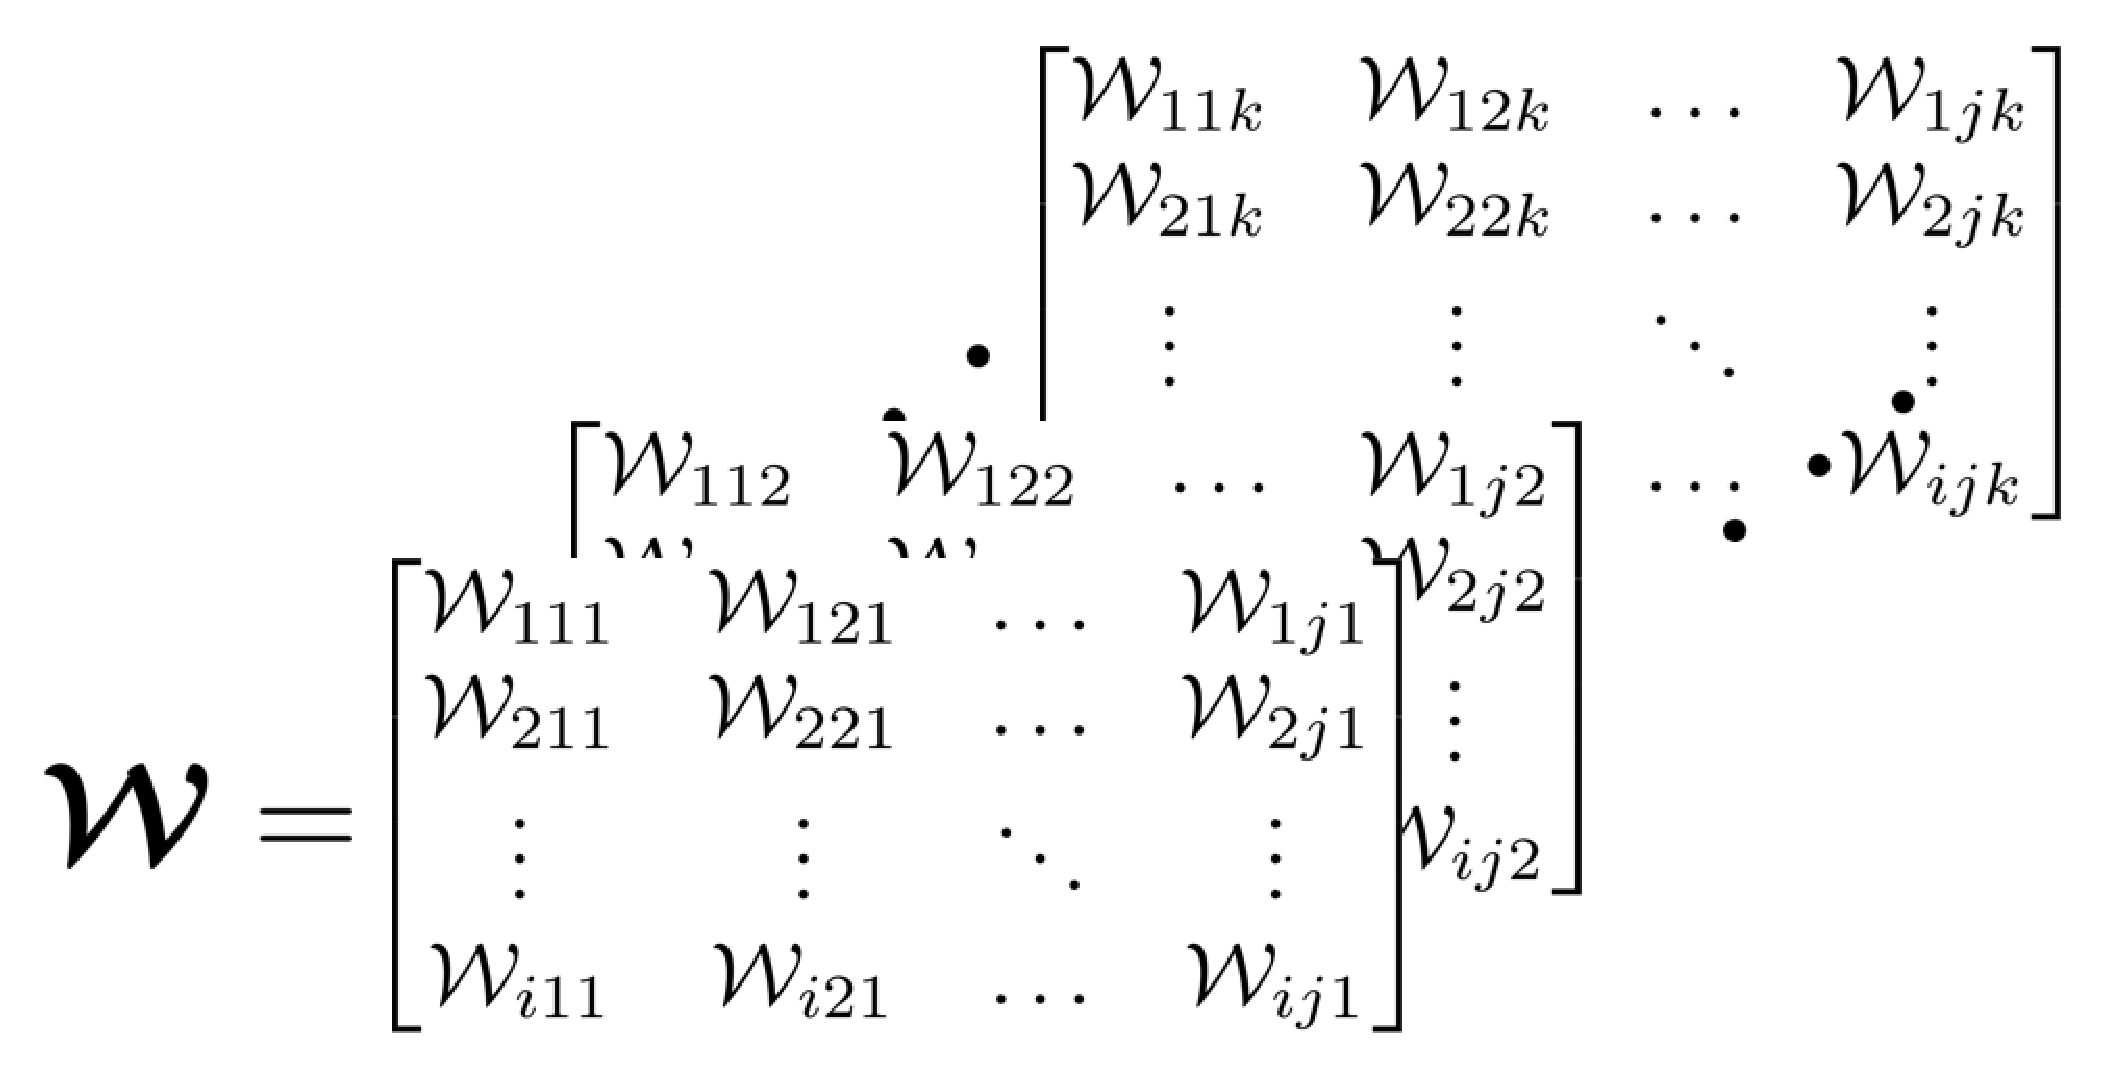
\includegraphics[width = 2.1in]{figures/abstract_matrix_rep.eps}
		\label{fig:abstract_matrix_rep}
	\end{center}
\end{figure}

Let us now define the total solution space, $\boldsymbol{\mathcal{S}}$, to be the set of all possible configurations of $\boldsymbol{\mathcal{W}}$ for a given neural network. In the synaptic weight selection problem domain it is more evocative to call $\boldsymbol{\mathcal{S}}$ the weight space of the network, so this convention adopted throughout this paper. Given $\boldsymbol{\mathcal{S}}$, we define a cost function $ \mathcal{C}$ to be the mapping

\begin{equation*} \label{eq:cost_mapping}
\mathcal{C} : \boldsymbol{\mathcal{S}} \rightarrow \mathbb{R}.
\end{equation*}


Each possible synaptic weight configuration of $\boldsymbol{\mathcal{W}}$ then corresponds to some cost value $\mathcal{C}(\boldsymbol{\mathcal{W}})$. Thus $\mathcal{C}(\boldsymbol{\mathcal{W}})$ defines a cost surface embedded  in the weight space. The objective is now to find a synaptic weight configuration, $\boldsymbol{\mathcal{W}_{opt}}$ such that 

\begin{equation*} \label{eq:optimal_definition}
\mathcal{C}(\boldsymbol{\mathcal{W}}_{opt}) \leq \mathcal{C}\left( \boldsymbol{\mathcal{W}}\right) , \forall\left(  \boldsymbol{\mathcal{W}} \in \boldsymbol{\mathcal{S}}\right) .
\end{equation*}

With this framework in place, we can apply the techniques of CSA and FSA to transition from a randomly-selected initial state, $\boldsymbol{\mathcal{W}}_0$, to $\boldsymbol{\mathcal{W}}_{opt}$.



\subsection{Neighborhood Functions}
\label{scn:neighborhood_fuctions}

All variations of simulated annealing require the specification of a neighborhood function, which determines the way in which new states may be generated from the current state. Let us define a generic feed-forward neural network weight neighborhood function, $\mathcal{N}$, which operates on a weight-space configuration $\boldsymbol{\mathcal{W}}$, thereby changing it to some new configuration $\boldsymbol{\mathcal{W}}'$. In the following section we detail several possible realizations of $\mathcal{N}$, some of which constitute an approximation to system performing quantum tunneling under the influence of an annealable artificial temperature. We also present a physical analogy of neighborhood function dynamics. Each neighborhood function will be evaluated and compared in Sec.~\ref{scn:experiments_results}.


\subsubsection{Physical Interpretation of Neighborhood Functions}
\label{scn:physical_interpretation_simulated_annealing}



The simulated annealing algorithm can be thought of as a means to move a neural network around its cost surface in a way analogous with a condensed matter system cooling to a low energy state. When considering only the influence of classical thermal fluctuations in particle energy levels, the probability of a particle traversing a potential energy barrier height \begin{math} \Delta V \end{math} at a temperature \begin{math} T \end{math} is on the order of: \begin{equation} \label{eq:thermal_transistion_prob}
\mathcal{P}_{c} = e^{-\frac{\Delta V}{T}}.
\end{equation}

As discussed in Section~\ref{scn:lit_review}, classical simulated annealing converges to a global, rather than local, minimum only if it is given sufficient time to converge. The amount of time required is problem dependent, and is often unacceptably long. One way to solve this problem is to create a mechanism by which the system can tunnel out of local minima to nearby, lower-cost configurations, thus reducing the amount of time needed to guarantee convergence to the global minimum. This is analogous to the quantum mechanical phenomenon of tunneling. In a quantum tunneling event a particle with energy \begin{math} E \end{math} incident upon a potential energy barrier of height \begin{math} \Delta V > E  \end{math} has a non-zero probability of being found in, or past, the barrier. Classically, this behavior is forbidden. The probability of tunneling, \begin{math} \mathcal{P}_{q} \end{math}, through a step barrier of height \begin{math} \Delta V  \end{math} is described by: 
\begin{equation} \label{eq:quantum_transition_prob}
\mathcal{P}_{q} = e^{-\frac{w \sqrt{\Delta V}}{ \Gamma}} 
\end{equation}

\noindent where \begin{math} \Gamma \end{math} is the tunneling field strength \cite{mukherjee2015multivariatesearchqa}. Fig.~\ref{fig:quantum_tunneling} depicts a one-dimensional example of quantum tunneling.


\begin{figure}[ht!]
	
	\begin{center}
		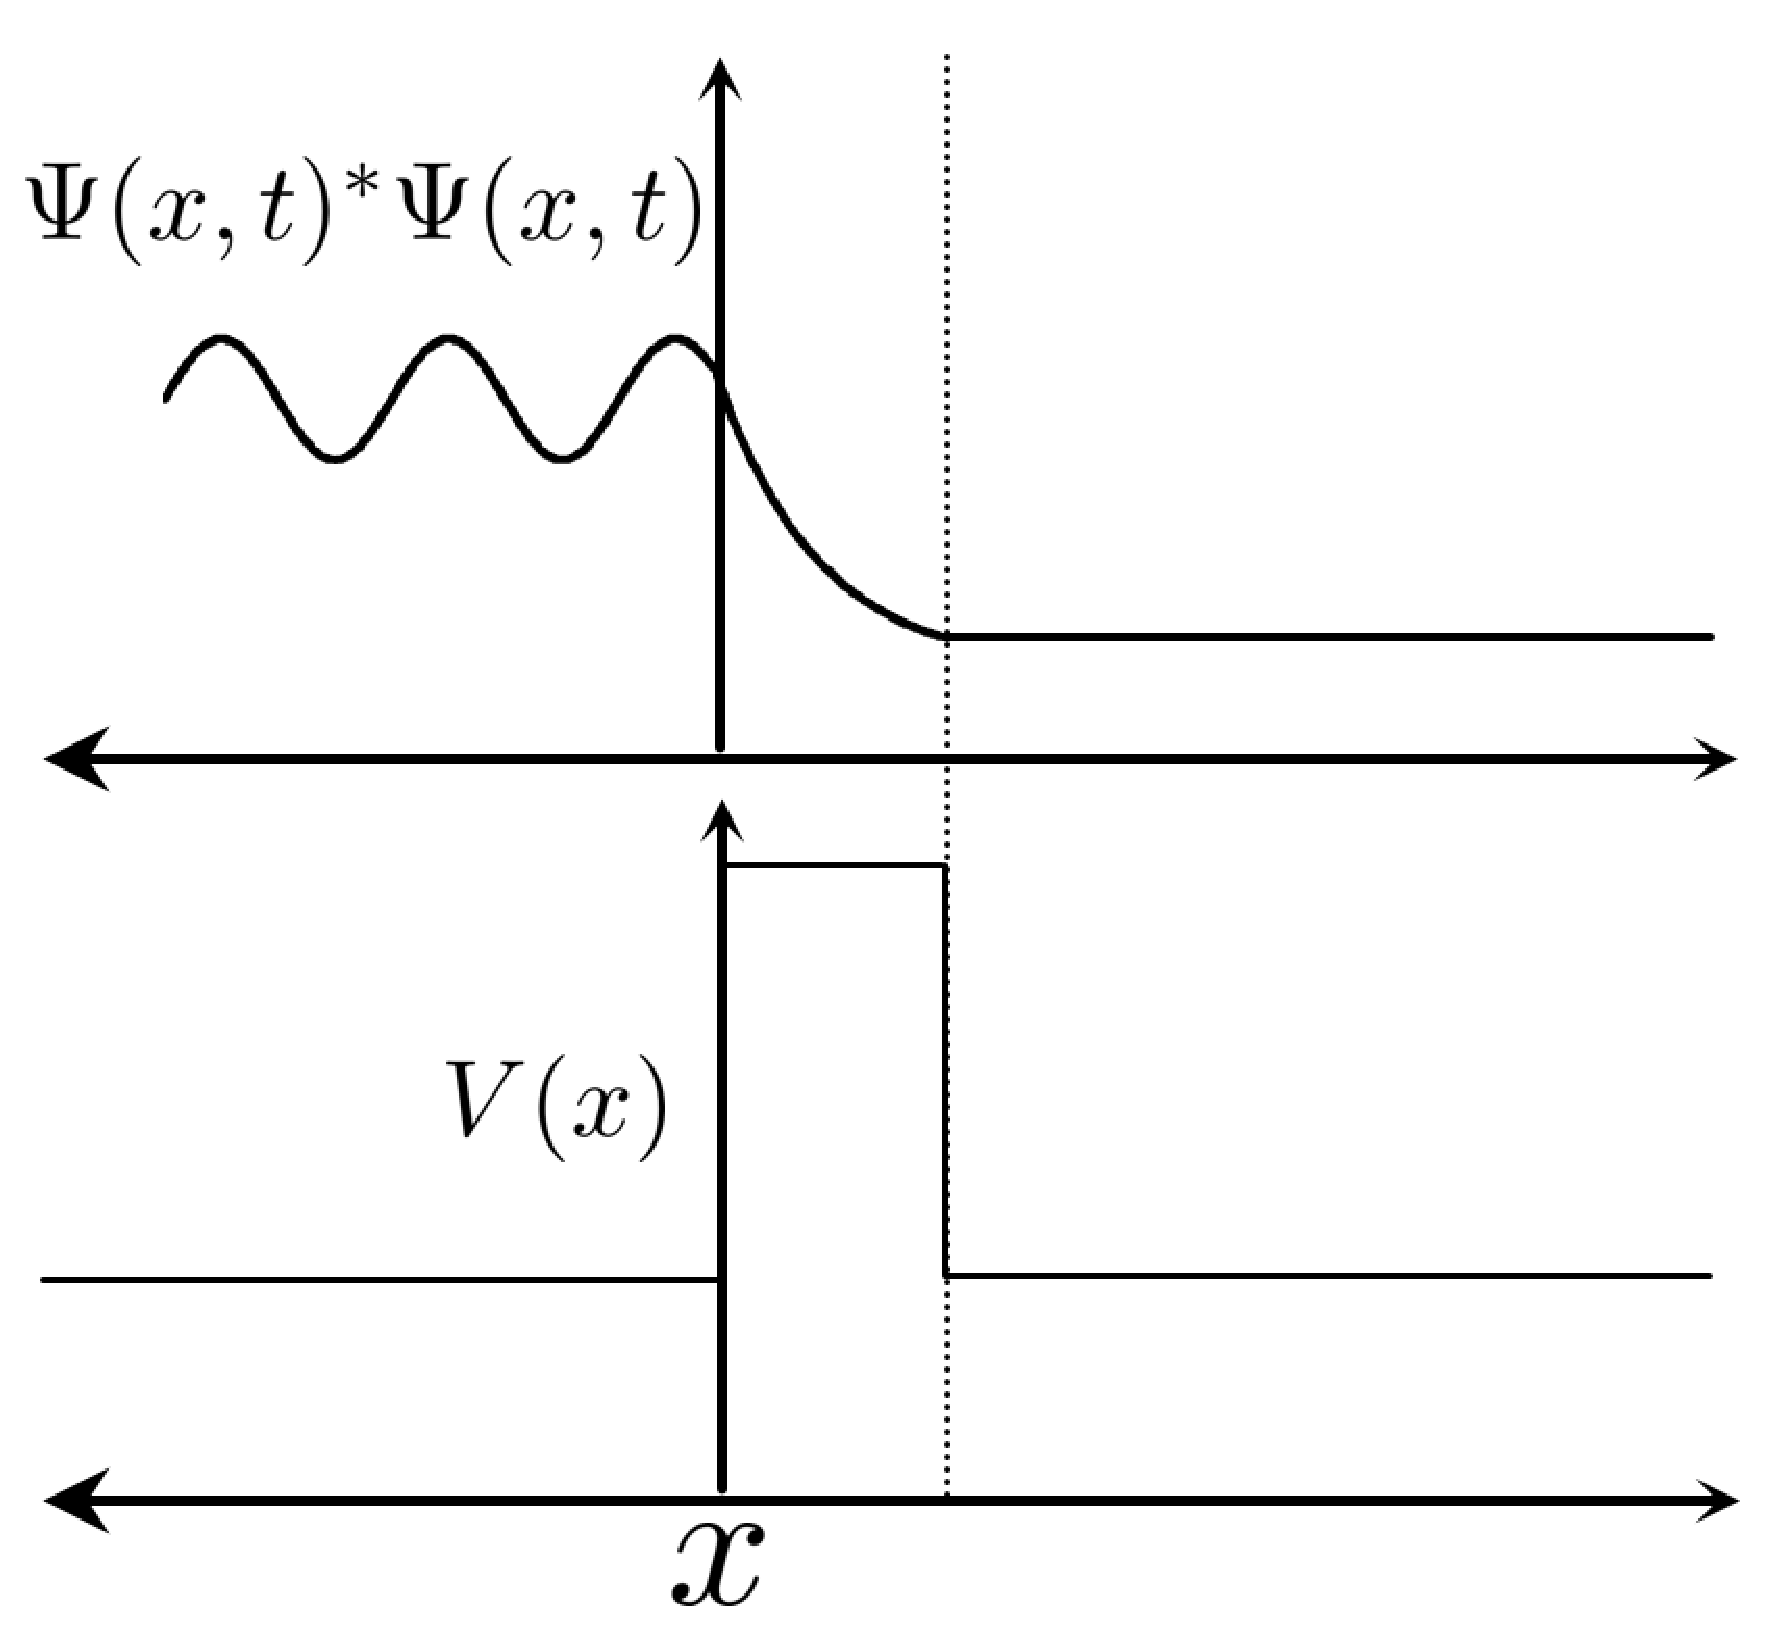
\includegraphics[width = 2.1in]{figures/tunneling_ex.eps}
	\end{center}
	\caption{(Bottom) A simple step potential in one dimension. (Top) The probability density function of a generic quantum system in the presence of a potential energy step barrier. There is an exponential decrease in probability through the barrier, and a uniform probability beyond the barrier.}
	
	\label{fig:quantum_tunneling}
\end{figure}


It is instructive to contrast Eq.~\ref{eq:thermal_transistion_prob} and Eq.~\ref{eq:quantum_transition_prob}. Both describe the same value, but the importance of the width and height of the traversed barrier in the two equations is considerably different. For systems in which quantum tunneling is possible, the probability of penetrating a barrier of height $\Delta V$ is increased by a factor of approximately $e^{\Delta V}$, for large values of $\Delta V$. This relationship is depicted graphically in Fig.~\ref{fig:quantum_advantage} which shows the probability of barrier traversal for a system which allows quantum fluctuations, divided by the same probability for a system which only considers thermal fluctuations. As can be seen in the figure, physical models which consider quantum effects are more likely predict penetration of tall, thin energy barriers than those which only include classical thermal effects. This tendency to allow the traversal of otherwise entrapping barriers reduces the likelihood of converging to a local minimum. Given that the cost, or error, surface of a neural network is likely to contain several local minima, an annealing system which incorporates quantum tunneling may outperform those that do not. The FSA algorithm presented in \cite{szu1987fastsimulatedannealing} is effectively a realization of this analogy to quantum mechanics. Unlike CSA, the FSA algorithm generates neighbor configurations which are sufficiently far from the current configuration that they may be on the other side of a cost surface barrier. 

\begin{figure}
	
	\begin{minipage}[b]{0.48\linewidth}
		\centering
		\centerline{\epsfig{figure=figures/quantum_advantage_a.eps,width=4.5cm}}
		%  \vspace{2.0cm}
		\centerline{(a)}\medskip
	\end{minipage}
	\hfill
	\begin{minipage}[b]{0.48\linewidth}
		\centering
		\centerline{\epsfig{figure=figures/quantum_advantage_b.eps,width=4.5cm}}
		%  \vspace{2.0cm}
		\centerline{(b)}\medskip
	\end{minipage}
	%\vspace{-0.5cm}
	\caption{
		(a) A potential energy barrier on a one-dimensional potential energy surface.
		(b) The tunneling probability relative to the probability of traversal due to thermal fluctuation for a step barrier plotted as a function of the height and width of the barrier.}
	\label{fig:quantum_advantage}
	%
\end{figure}



\subsubsection{Classical Neighborhood Functions}
\label{scn:classical_neighborhood}

We define \begin{math}\mathcal{N}_{c}\end{math} to be the classical neighborhood function for feed-forward neural network weights, which is defined as \begin{align}\label{eq:classical_anisotropic_neighborhood}
	\mathcal{N}_{c} (\boldsymbol{\mathcal{W}}) = \boldsymbol{\mathcal{W}} + \alpha g_{G}(u) \boldsymbol{\mathcal{A}} 
\end{align}
\noindent where $\alpha$ is the learning rate, $g_{G}(u)$ is a Gaussian generating function, $u$ is a uniform random variable over the range $U[0,1]$, and $\boldsymbol{\mathcal{A}}$ is a matrix with dimensionality equal to that of $\boldsymbol{\mathcal{W}}$. Each element of $\boldsymbol{\mathcal{A}}$ is generated from a distribution over the range $[-1,1]$.  $\boldsymbol{\mathcal{A}}$ is restricted such that for each element of $\boldsymbol{\mathcal{W}}$ that is zero the corresponding element in $\boldsymbol{\mathcal{A}}$ is zero, and that $\boldsymbol{\mathcal{A}}$ must be normalized such that the magnitude of the matrix elements sum to $1$. These restrictions ensure two useful properties of the classical neighborhood function, that: 

\begin{enumerate}
	\item $\mathcal{N}_{c} (\boldsymbol{\mathcal{W}})$ will produce a weight matrix, $\boldsymbol{\mathcal{W}'}$, which will have an $L^2$ distance of exactly $\alpha g_{G}(u)$ from the original matrix, $\boldsymbol{\mathcal{W}}$, in the weight space. Said differently, no matter how the total change in the weight matrix is distributed among the weights, the total distance of the change is conserved.
	\item This traversal distance will be distributed anisotropically over the weights, with the anisotropicity determined by the distribution used to generate $\boldsymbol{\mathcal{A}}$. (See Sec.~\ref{scn:anisotropicity} for more information.)
\end{enumerate}
These properties are useful in that they allow for strict control over the systems traversal of the cost surface, and the decouple the implementations of the visiting distribution and anisotropicity.

The neighborhood function given in Eq.~\ref{eq:classical_anisotropic_neighborhood} is an application of the canonical form of simulated annealing to the problem of selecting a weight configuration for a feed-forward neural network. The term classical is used here because the underlying simulated annealing model can be described entirely in terms of classical statistical mechanics. To interpret this in terms of the analogy present in Sec.~\ref{scn:physical_interpretation_simulated_annealing}, the probability of the Gaussian visiting distribution used in CSA generating a weight space distance large enough to transition the system across a large energy barrier is effectively $0$. In the next section, a model which approximates quantum mechanical phenomena will be constructed.

\subsubsection{Quantum-Inspired Neighborhood Functions}
\label{scn:quantum_neighborhood}

The classical neighborhood function present in Sec.~\ref{scn:classical_neighborhood} is one of many which could be employed in CSA. In order to incorporate quantum tunneling into this model, we must have some mechanism which allows the neighborhood function to generate neighbor states which are across a cost surface barrier. Since it is impossible to know the cost function value of a configuration which has not yet been evaluated, we must construct a neighborhood function which is able to jump to these configurations. This mechanism is often called a trial jump. We define our quantum neighborhood function for feed-forward neural network weights to be
\begin{align}\label{eq:quantum_anisotropic_neighborhood}
\mathcal{N}_{q} (\boldsymbol{\mathcal{W}}) = \boldsymbol{\mathcal{W}} + \alpha g_{q}(u) \boldsymbol{\mathcal{A}} 
\end{align}
\noindent where $\alpha$, $u$, and $\boldsymbol{\mathcal{A}}$ are defined as they are in Eq.~\ref{eq:classical_anisotropic_neighborhood}, and $g_{q}(u)$ is a parameterized generation function used to produce a value from the visiting distribution. As in \cite{tsallis1996generalizedsimulatedannealing}, the visiting distribution is defined as the probability distribution function of the trial jump distance. 

Several visiting distributions may be used used to approximate quantum tunneling in order to form a quantum neighborhood function, $g_{q}$. The most obvious choice is the exponential distribution, for which the generation function is given by
\begin{align}\label{eq:exp_generation_fcn}
g_{e}(u) =  \frac{-\ln(u)}{\gamma}
\end{align}
\noindent where $\gamma$, the scale parameter for the distribution, is defined as $\Gamma$. The exponential distribution closely aligns with physical reality, as the probability of penetrating a barrier decreases exponentially with the barriers width. This can be seen in Eq.~\ref{eq:quantum_transition_prob} and Fig.~\ref{fig:quantum_tunneling}. The barrier width in Eq.~\ref{eq:quantum_transition_prob} and Fig.~\ref{fig:quantum_tunneling} is analogous to the trial jump distance in the quantum neighborhood function. The introduced stochastic control parameter $\Gamma$ denotes the strength of the tunneling field as in \cite{mukherjee2015multivariatesearchqa}, and thus controls the likelihood of a long trial jump. $\Gamma$ is supported on $[0,1]$. A large value of $\Gamma$ corresponds to frequent, long range quantum trial jumps. It is the stochastic control parameter $\Gamma$ value that connects the quantum neighborhood function to quantum annealing. Much like FSA \cite{szu1987fastsimulatedannealing}, this provides mostly local search with occasional global-scale searches. Other generating functions corresponding to other visiting distributions may also be used to generate new states. 

In FSA the Cauchy distribution is used as the visiting distribution. The generation function for the Cauchy distribution is

\begin{align}\label{eq:cauchy_generation_fcn}
g_{C}(u) =  c \tan\left(u-\frac{1}{2}\right)
\end{align}

\noindent where $c$ is the shape parameter of the Cauchy distribution used for the visiting distribution. We set $c$ to be $1/(1-\Gamma)$, which ensures that $g_{C}(u) \rightarrow u \left| \boldsymbol{\mathcal{S}}\right| $, where $\left| \boldsymbol{\mathcal{S}}\right|$ is the total size of the configuration space, in the $\Gamma \rightarrow 1$ limit. That is, as $\Gamma$, the stochastic control parameter for tunneling, goes to it's maximum value, $g_{C}(u)$ approaches the uniform distribution, thereby allowing tunneling of any distance.


Finally, we consider the case of the uniform visiting distribution, which has an equal probability of visiting any possible configuration in the solution space. Inspecting Fig.~\ref{fig:quantum_tunneling} we see that the probability of tunneling to any location past the step potential energy barrier is uniform\footnote{The quantum mechanical analogy is intentionally incomplete here. Strictly speaking, the probability is only uniform over the entire cost surface if no other barriers exist on the surface} . If we assume that every cost surface barrier encountered by the algorithms is small relative to the size of the complete cost surface, it is not unreasonable to approximate the probability of transition to any state as uniform. The generation function for this distribution is given by

\begin{align}\label{eq:uniform_generation_fcn}
g_{U}(u) = (g_{G}(u) +  u \left| \boldsymbol{\mathcal{S}} \right| (\Gamma\geq u))
\end{align}
\noindent which results in a trial jump to any location in the configuration space, but only with probability equal to $\Gamma$. In the case where a uniform trial jump does not occur, $g_{U}(u)$ reduces to $g_{G}(u)$. In other words, in the $\Gamma \rightarrow 0$ limit, CSA is recovered.

\subsubsection{Anisotropicity}
\label{scn:anisotropicity}
In the course of developing the synaptic weight selection system presented in this paper, it was observed that it is sometimes advantageous to move along an error surface in a relatively small subset of the total number of dimensions. Such a modification of the configuration corresponds to the modification of a single synaptic weight in a training epoch. Though it is possible that this could occur by chance, the likelihood of a single-weight modification is inversely proportional to the number of weights in the network. For large networks this probability becomes vanishingly small, so a mechanism is introduced to increase the frequency of occurrence of these fine-tuning events. In the physical science a directionally-dependent event, one that varies differently in some subset of its degrees of freedom, is called an anisotropy. Thus, an anisotropicity matrix, $\boldsymbol{\mathcal{A}}$, which indicates how much of a given configuration change will be applied to each of the weights, which are analogous to degrees of freedom in the neural network configuration. The restrictions described in Sec.~\ref{scn:classical_neighborhood} hold. In this section we turn our attention to the mechanism used to generate the distribution of values in $\boldsymbol{\mathcal{A}}$. 

The simplest possible realization of $\boldsymbol{\mathcal{A}}$ is the isotropic limit. In this case the total $L^2$ distance traversed through the weight space is distributed evenly among the weights. We denote the anisotropicity matrix corresponding to this case as
\begin{align}\label{eq:isotropic_anisotropicity}
\boldsymbol{\mathcal{A}}_0 = \frac{1}{D}  \boldsymbol{J}_{\pm}
\end{align}
\noindent where $D$ is the number of non-zero elements in $\boldsymbol{\mathcal{W}}$, and $\boldsymbol{J}_{\pm}$ is a unit matrix of equal dimensionality to $\boldsymbol{\mathcal{W}}$ in which each element is randomly and with equal probability assigned a sign. This definition of anisotropicity scales the step size inversely with the number of synaptic connection in the matrix. In very large matrices, this is problematic because the change in each individual synaptic weight becomes so small that the change in weight value produces effectively no change in the cost function value, thus causing the cost surface to flatten. In practice, we observe that it is possible to counteract this gradient dilution by simply scaling the anisotropicity matrix by the number of synapses in the network. For the isotropic anisotropicity matrix, this scaling yields
\begin{align}\label{eq:isotropic_anisotropicity_scaled}
\boldsymbol{\mathcal{A}}_0 =  \boldsymbol{J}_{\pm}.
\end{align} 

The isotropic weight space traversal implied by $\boldsymbol{\mathcal{A}}_0$ is equal in distance for all synaptic weights, with only the direction of the change varying among the weights. Though this weight modification policy is sufficient to train classification networks, there is relatively little diversity of ways in which the synaptic weights can change. A natural extension of $\boldsymbol{\mathcal{A}}$ which allows for greater diversity of synaptic weight modification, is to allow the portion of the total weight matrix change contributed by each synaptic weight to be randomly chosen. We define the anisotropicity matrix which implements this extension as

\begin{align}
	\boldsymbol{\mathcal{A}}_U =  \frac{\boldsymbol{U}}{D/2}
\end{align}

\noindent where $\boldsymbol{U}$ is a matrix of dimensionality equivalent to $\boldsymbol{\mathcal{W}}$ for which each element is drawn from $U[0,1]$.  The denominator ensures statistical compliance with the restriction that the elements of any matrix used as a realization of $\boldsymbol{\mathcal{A}}$ sum to unity. This constrain is very likely to be satisfied by $\boldsymbol{\mathcal{A}}_U$ for large networks because $\left\langle  U[0,1] \right\rangle =1/2$. Therefore, because there are $D$ non-zero elements in $\boldsymbol{U}$ the expectation value of the sum of the elements in $\boldsymbol{U}$ is $D/2$. Applying the same dimensional scaling as in Eq.~\ref{eq:isotropic_anisotropicity_scaled} and simplifying, we find that

\begin{align}
\boldsymbol{\mathcal{A}}_U =  2 \boldsymbol{U}.
\label{eq:uniform_anisotropicity}
\end{align}

Using $\boldsymbol{\mathcal{A}}_U$ yields significantly more diversity of synaptic weight perturbations, but there is still a large class of possible perturbations which it is very unlikely to generate. These perturbations are those in which a large portion of the synaptic weights are left unchanged while some subset is changed significantly. In order to create a realization of $\boldsymbol{\mathcal{A}}$ which generates this type of perturbation we introduce a new stochastic control parameter, $\kappa$, which specifies the concentration of the total anisotropicity and is supported on the range $(0, 1/4)$. Thus, the anisotropicity of the matrix varies with the value of  $\kappa$. We define the variable anisotropicity matrix to be


\begin{align}
\boldsymbol{\mathcal{A}}_V =  2^{\frac{1}{1-\kappa}} \cdot power\left(\boldsymbol{U}, {\frac{1}{1-\kappa}}\right).
\end{align}

\noindent where the $power$ function is the element-wise scalar exponentiation function. This definition is already scaled and simplified, as in Eq.~\ref{eq:uniform_anisotropicity}. It is clear that in the $\kappa \rightarrow 0$ limit $\boldsymbol{\mathcal{A}}_U$ is recovered. In the $\kappa \rightarrow 1/4$ limit, the matrix has only a few large elements, with the rest set nearly to zero. The upper bound of $\kappa$ was determined empirically to be the largest value that does not result in a matrix which violates any of the constraints.

\subsection{Cost Function}
\label{scn:cost_functions}

We focus our analysis in this paper on the classification performance feed-forward neural networks. As such, we adopt the mean classification error cost function, defined average number of samples in a given data set for which the predicted classification label is different than the correct classification label.


\subsection{Annealing Schedules}
\label{scn:annealing_schedules}

The annealing schedule controls the way in which the stochastic control parameters change thorough simulation time. 

\subsubsection{Classical Simulated Annealing}
The canonical classical annealing schedule is given by  
\begin{align}
	T(t) = \frac{T_i}{\ln(t)}
\end{align}
\noindent where $t$ is the simulation time steps completed. This inverse-logarithmic decay statistically guarantees convergence to a global minimum if the system is allowed to reach a value of $T$ which is nearly $0$. Proof of this claim is presented in \cite{geman1984stochasticrelaxation}.

\subsubsection{Fast Simulated Annealing}
FSA is able to converge much more quickly to a global minimum due to it's ability to traverse large cost surface barriers, which would otherwise entrap CSA. Its temperature schedule is given by
\begin{align}
T(t) = \frac{T_i}{t}
\end{align}
\noindent where $t$ is the simulation time steps completed. Again, this decay is necessary and sufficient to ensure the system reached a global minimum in the $T \rightarrow 0$ limit \cite{szu1987fastsimulatedannealing}. 


%[If I had more propblems, with similiar results I would say: "It seems that the conclusions generalize well, as they appear to apply equally to all problems present in this work."]

\subsection{Synaptic Annealing Algorithm}

Given the components described in the preceding sections, we can now construct a complete algorithm for applying a general simulated annealing method to the problem of feed-forward neural network weight selection.

\begin{algorithm}
	\caption{Synaptic Annealing}
	\label{alg:synaptic annealing}
	\begin{algorithmic}
		\STATE $\boldsymbol{\mathcal{W}} \leftarrow \boldsymbol{\mathcal{W}}_0$
		\STATE $t \leftarrow 0$
		\WHILE{$T(t) > \epsilon$}
			\STATE $\boldsymbol{\mathcal{W}}' \leftarrow \boldsymbol{\mathcal{W}} + \alpha g(u) \boldsymbol{\mathcal{A}} $
			\STATE $\Delta C \leftarrow (\mathcal{C}(\boldsymbol{\mathcal{W}}')-\mathcal{C}(\boldsymbol{\mathcal{W}}))$
			\IF{$\Delta C \leq 0 $}
				\STATE $\boldsymbol{\mathcal{W}} \leftarrow \boldsymbol{\mathcal{W}}'$
			\ELSE [$ \exp(\Delta C/T(t) ) > U\left( 0,1\right)  $]
				\STATE $\boldsymbol{\mathcal{W}} \leftarrow \boldsymbol{\mathcal{W}}'$
			\ENDIF
			\STATE $t \leftarrow t+1$
		\ENDWHILE
		\STATE $\boldsymbol{\mathcal{W}}_{opt} \leftarrow \boldsymbol{\mathcal{W}}$
		\RETURN $(\boldsymbol{\mathcal{W}}_{opt})$
	\end{algorithmic}
\end{algorithm}

\section{Experiments and Results}
\label{scn:experiments_results}
\makeatletter
\def\fixedlabel#1#2{%
	\@bsphack%
	\protected@write\@auxout{}%
	{\string\newlabel{#1}{{#2}{\thepage}}}%
	\@esphack}
\makeatother

\begin{figure*}[ht!]
	\centering
	\setlength{\tabcolsep}{-3pt}
	\begin{tabular}{c@{}cccc}
		& Gaussian & Exponential & Cauchy & Uniform \\
		
		\rotatebox{90}{Isotropic }
		& 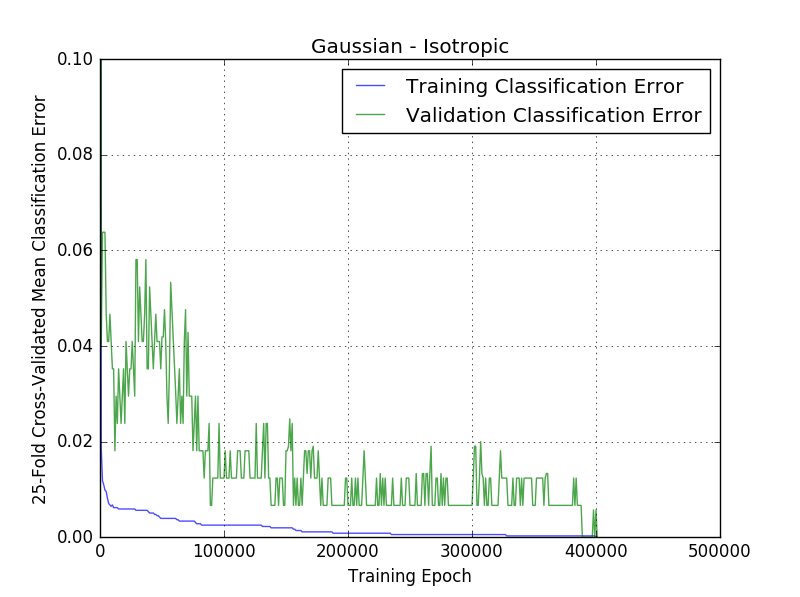
\includegraphics[width = 1.8in, trim={0.5cm 0 1.3cm 0.8cm},clip]{figures/classPerf/classPerf_g_i.png} \fixedlabel{block1a}{1a} 	
		& 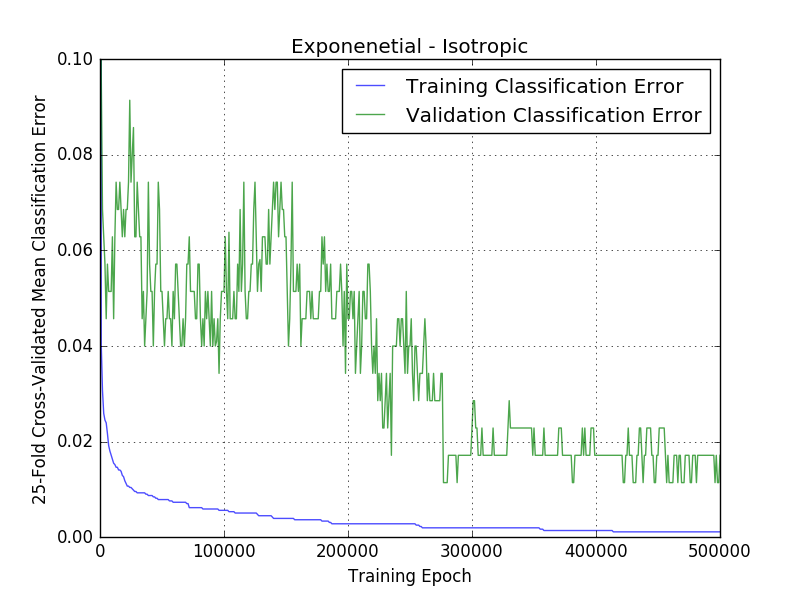
\includegraphics[width = 1.6in, trim={2.35cm 0 1.5cm 0.8cm},clip]{figures/classPerf/classPerf_e_i.png} \fixedlabel{block1b}{1b} 
		& 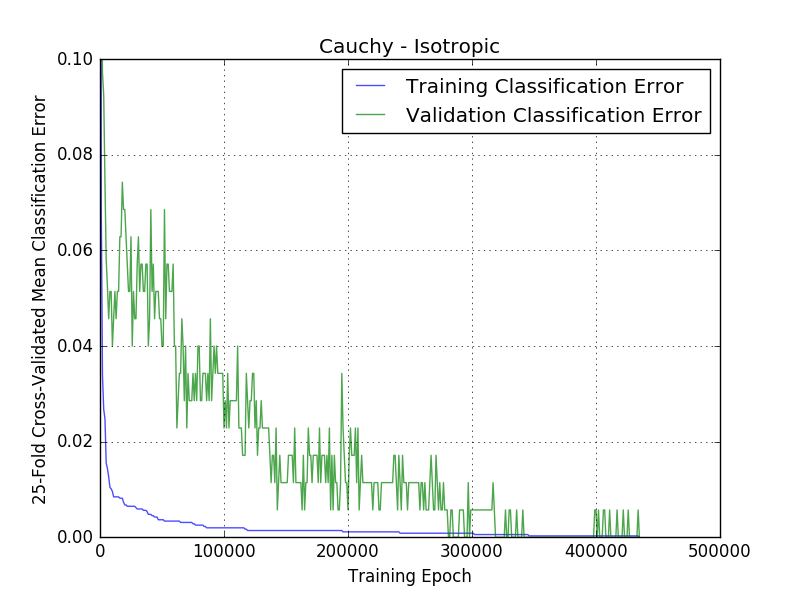
\includegraphics[width = 1.6in, trim={2.35cm 0 1.5cm 0.8cm},clip]{figures/classPerf/classPerf_c_i.png} \fixedlabel{block1c}{1c} 
		& 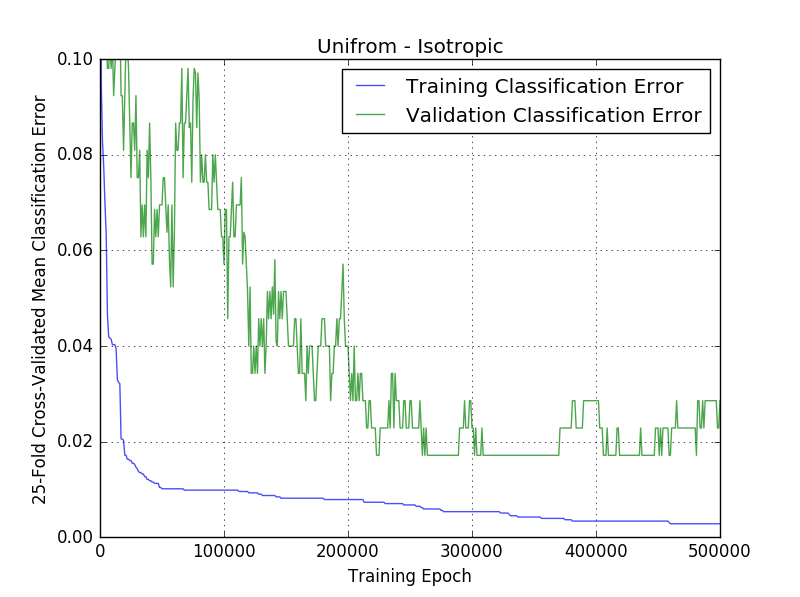
\includegraphics[width = 1.6in, trim={2.35cm 0 1.5cm 0.8cm},clip]{figures/classPerf/classPerf_u_i.png} \fixedlabel{block1d}{1d} \\ \\[-10pt]
		
		
		\rotatebox{90}{	\begin{tabular}[x]{@{}c@{} }   Uniform \\ Anisotropicity \end{tabular} }
		& 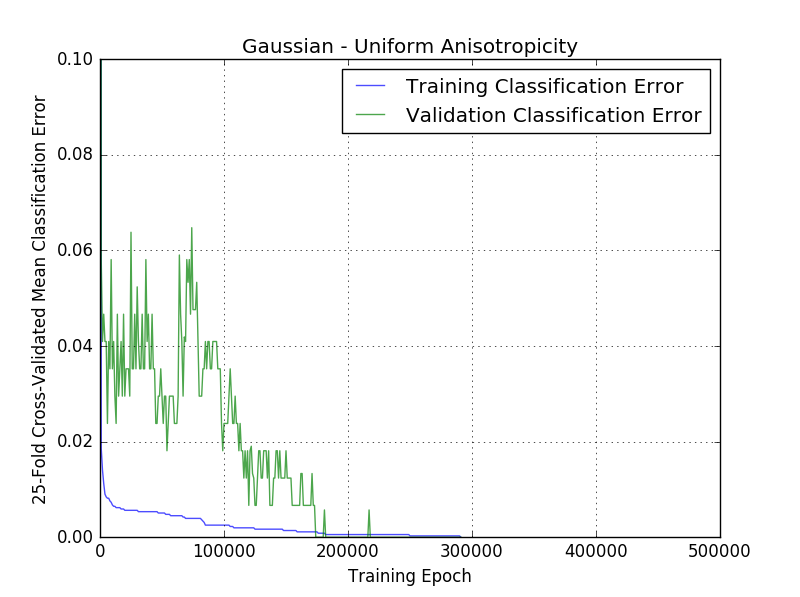
\includegraphics[width = 1.8in, trim={0.5cm 0 1.3cm 0.8cm},clip]{figures/classPerf/classPerf_g_ua.png} \fixedlabel{block2a}{2a} 
		& 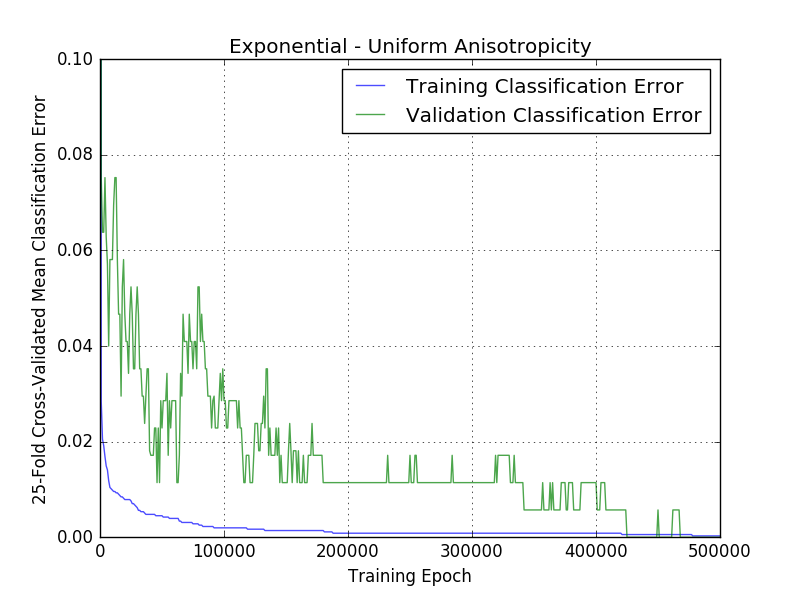
\includegraphics[width = 1.6in, trim={2.35cm 0 1.5cm 0.8cm},clip]{figures/classPerf/classPerf_e_ua.png} \fixedlabel{block1b}{2b} 
		& 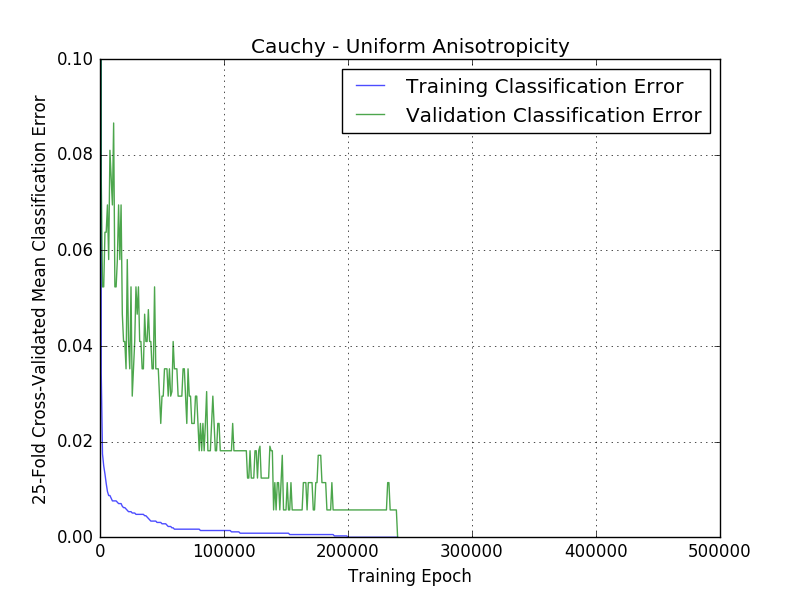
\includegraphics[width = 1.6in, trim={2.35cm 0 1.5cm 0.8cm},clip]{figures/classPerf/classPerf_c_ua.png} \fixedlabel{block1b}{2c} 
		& 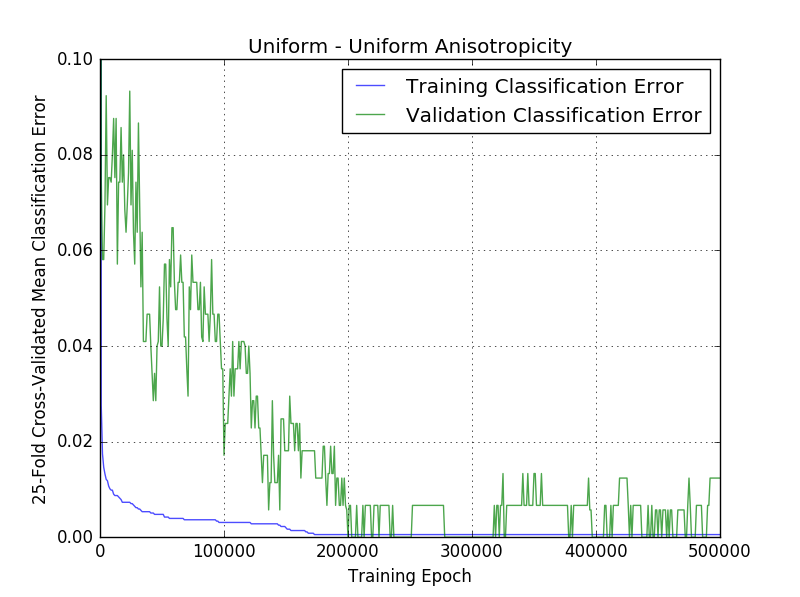
\includegraphics[width = 1.6in, trim={2.35cm 0 1.5cm 0.8cm},clip]{figures/classPerf/classPerf_u_ua.png} \fixedlabel{block2b}{2d} \\ \\[-10pt]
		
		\rotatebox{90}{	\begin{tabular}[x]{@{}c@{}} Variable \\ Anisotropicity \end{tabular}	}
		& 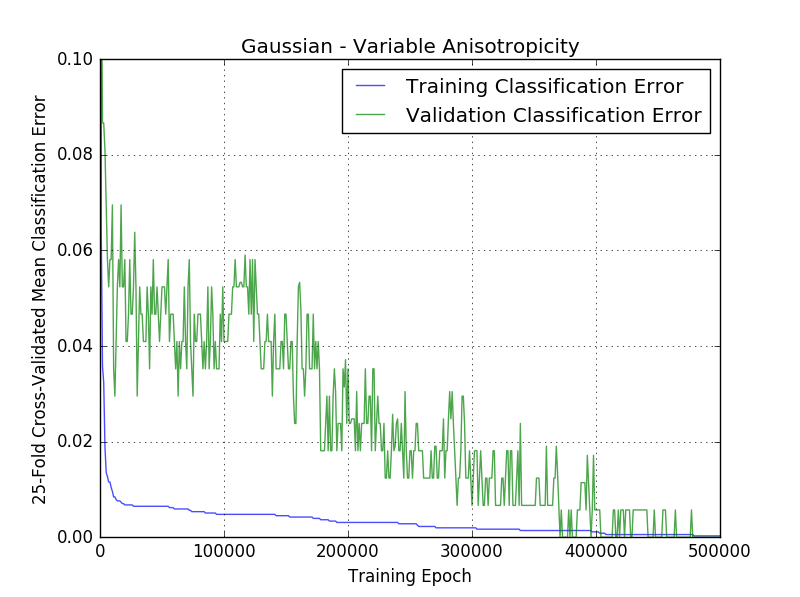
\includegraphics[width = 1.8in, trim={0.5cm 0 1.3cm 0.8cm},clip]{figures/classPerf/classPerf_g_va.png}\fixedlabel{block3a}{3a} 
		& 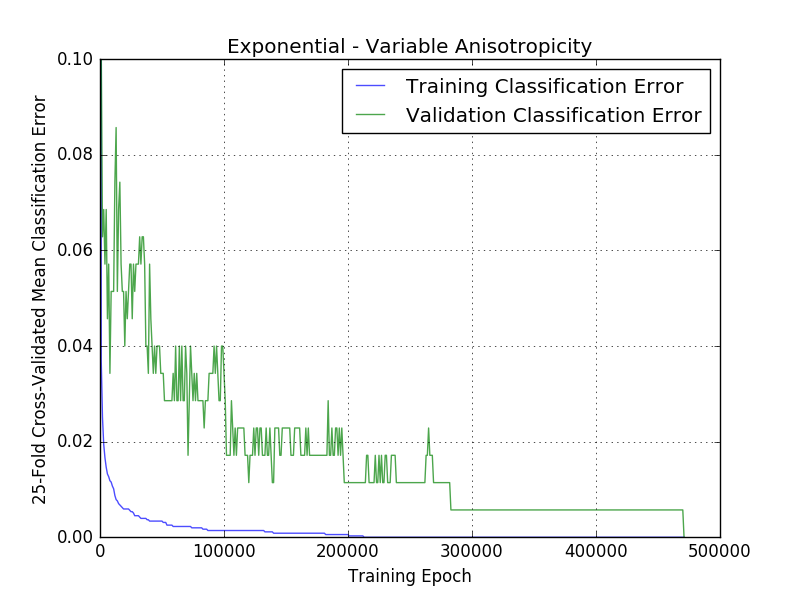
\includegraphics[width = 1.6in, trim={2.35cm 0 1.5cm 0.8cm},clip]{figures/classPerf/classPerf_e_va.png}\fixedlabel{block1b}{3b} 
		& 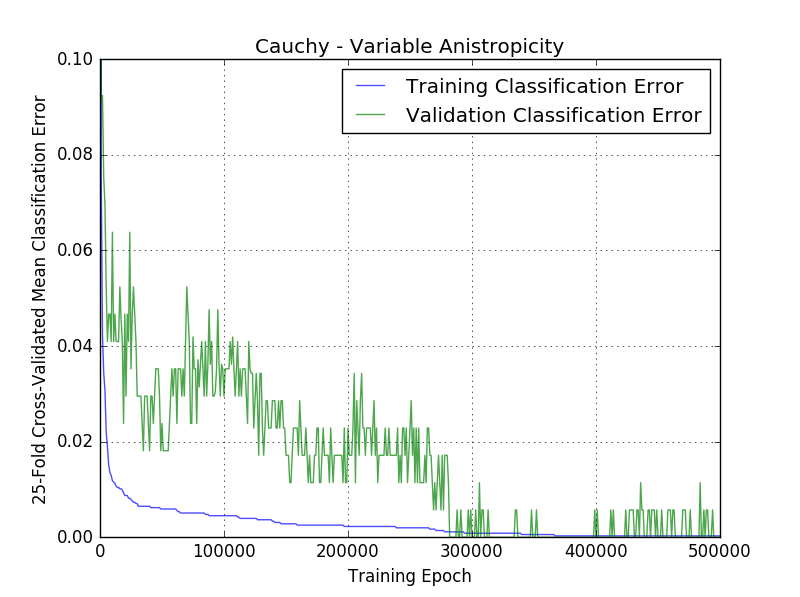
\includegraphics[width = 1.6in, trim={2.35cm 0 1.5cm 0.8cm},clip]{figures/classPerf/classPerf_c_va.png}\fixedlabel{block1b}{3c} 
		& 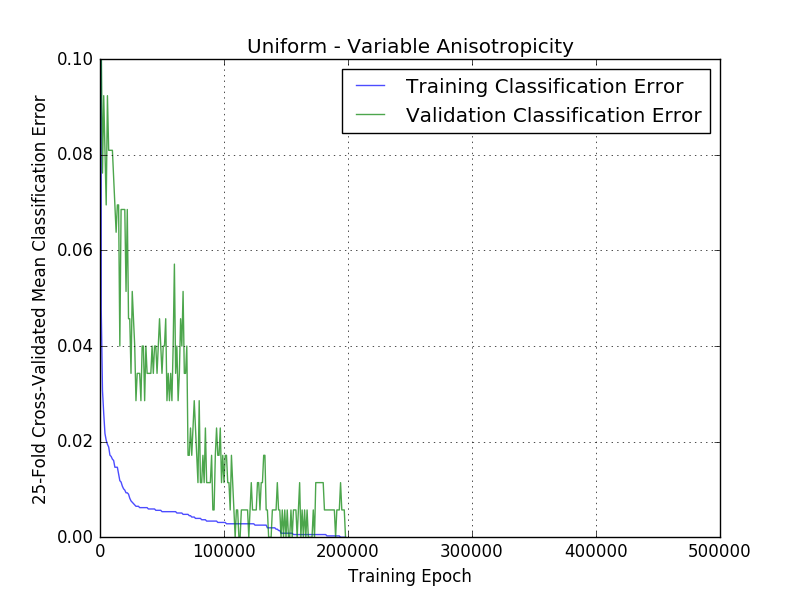
\includegraphics[width = 1.6in, trim={2.35cm 0 1.5cm 0.8cm},clip]{figures/classPerf/classPerf_u_va.png}\fixedlabel{block3b}{3d}
		
	\end{tabular}
	\caption{The simulation-time evolution of the 25-fold cross-validated classification error of a feed-forward neural network with 50 hidden units on Fishers iris data. Each column in this table depicts the results for an SA neighborhood function employing a single type of visiting distribution, which is indicated in the column header. Each row depicts a single type of anisotropicity strategy, which is indicated in the row header. The classification error is defined as the fraction of samples incorrectly classified.}
	
	\label{fig:class_perf}
	
\end{figure*}


In this section several experiments are presented to evaluate the performance of the annealing procedures defined in the Sec.~\ref{scn:problem_formulation}.


\subsection{Classification Performance}

We begin by evaluating the impact of neighborhood function choice on the classification performance of a feed-forward neural network trained by SA. Fig.~\ref{fig:class_perf} contains the simulation-time evolution of classification performance for a feed-forward neural network with 50 hidden units in a single hidden layer. This performance data was generated by a neural network trained to classify Fishers iris data, which comprises $150$ samples with input dimensions and $3$ class labels. Before training on the data, it is normalized, shuffled and the mean is removed.

Each experiment, which consists of the evaluation of a single neighborhood function, is performed using 25-fold cross validation. The results presented in Fig.~\ref{fig:class_perf} are the time evolution of the mean training and validation set classification error. All results are presented up to the $500,000$\textsuperscript{th} training epoch. Each training epoch evaluates the entire training and validation set when producing the classification error.


\subsubsection{Visiting Distribution Analysis}

The classification performance of CSA, which is defined by an isotropic application of a Gaussian generating function, is displayed in the top-left tile of \ref{fig:class_perf}. We see that 25-fold cross validated perfect classification is achieved at approximate $400,000$ epochs. That is, all 25 of the independent SA trials had achieved perfect classification at or before epoch $400,000$. Comparing the only the performance of the isotropic anisotropicity neighborhood functions we find that the Cauchy visiting distribution converged slightly faster than the Gaussian on the training set, but takes slightly longer to correctly generalize to the validation set. This is somewhat unexpected, as FSA is generally much faster than CSA. The exponential visiting distribution performs poorly relative to both CSA and FSA, but this is not surprising. Though the exponential distribution is in close analogy to the physics of quantum tunneling it is a very light-tailed function, and as such is unlikely to produce neighbors far from the current configuration. As such, it appears to be unable traverse the error surface as quickly. Finally, we find that the worst performing visiting distribution is the uniform distribution. The uniform visiting distribution amounts to a random global search of the weight space; the weight space for this problem is $350$-dimensional, so finding the global minimum of the space by chance is unlikely. These performance relationships between visiting distribution hold for all anisotropicity strategies, with the notable exception of uniform visiting distributions with variable annealing, which is discussed in Sec.~\ref{scn:anisotropicity_analysis}

\subsubsection{Anisotropicity Analysis}
\label{scn:anisotropicity_analysis}

Observing figs.~\ref{fig:class_perf} and \ref{fig:perfect_class_time} we see that neighborhood functions implementing uniform anisotropicity consistently outperform those which use isotropic weight change assignment. Further, we find that while variable anisotropicity confers no advantage on either CSA or FSA, it significantly improves the performance of the two non-canonical simulated annealing visiting distributions. With variable anisotropicity, both the exponential and uniform distribution outperform CSA and FSA. One of the most striking results depicted in Fig.~\ref{fig:perfect_class_time} is the interaction effect of a uniform visiting distribution and a variable anisotropicity matrix, visible in the bottom-right corner of the figure. While both the uniform visiting distribution and the variable anisotropicity under-perform relative to their alternatives, when combined the make for the most effective neighborhood function considered in this paper. This interaction effect is likely due to the specificity of modification afforded by the combination of a highly anisotropic modification and a global search reach. We should expect that for very large networks this advantage would diminish somewhat, as the global search space would be much larger. Further study is needed to evaluate the potential general applicability of this neighborhood function.


\begin{figure*}
	\label{fig:perfect_class_time}
	\centering
	\setlength{\tabcolsep}{-3pt}
	\begin{tabular}{c@{}cccc}
		& Gaussian & Exponential & Cauchy & Uniform \\
		
		\rotatebox{90}{Isotropic }
		& 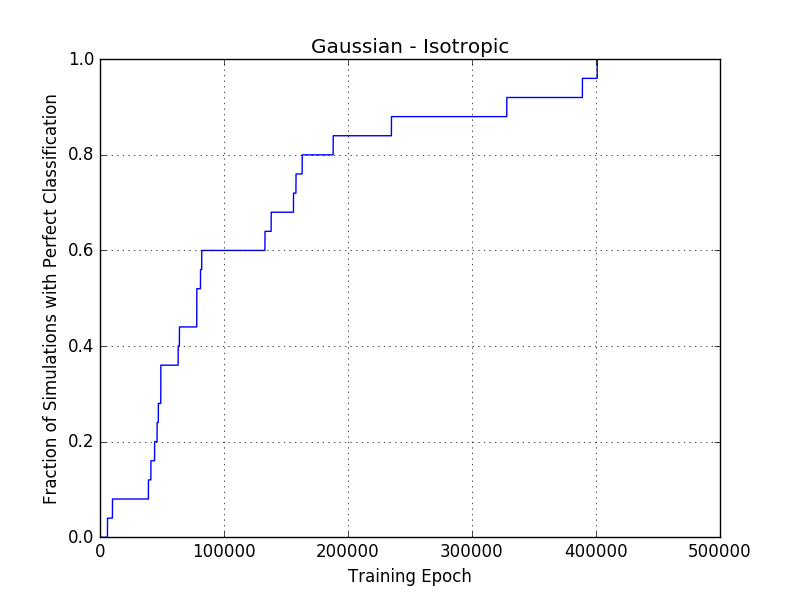
\includegraphics[width = 1.8in, trim={0.5cm 0 1.3cm 0.8cm},clip]{figures/completeFrac/completeFrac_g_i.png} \fixedlabel{block1a}{1a} 	
		& 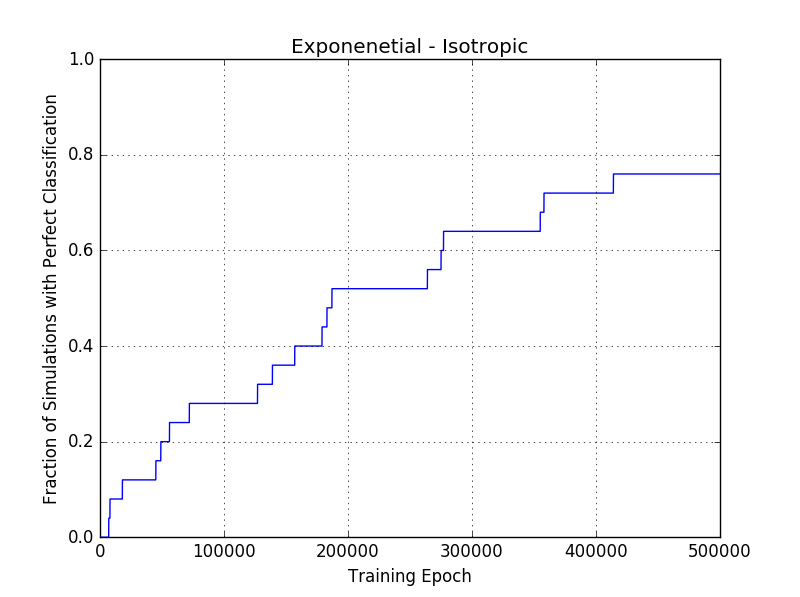
\includegraphics[width = 1.6in, trim={2.35cm 0 1.5cm 0.8cm},clip]{figures/completeFrac/completeFrac_e_i.png} \fixedlabel{block1b}{1b} 
		& 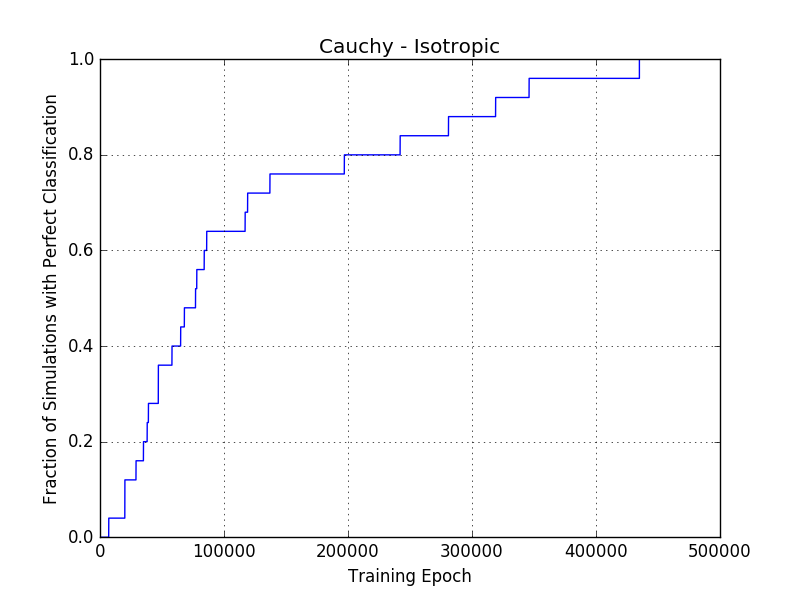
\includegraphics[width = 1.6in, trim={2.35cm 0 1.5cm 0.8cm},clip]{figures/completeFrac/completeFrac_c_i.png} \fixedlabel{block1c}{1c} 
		& 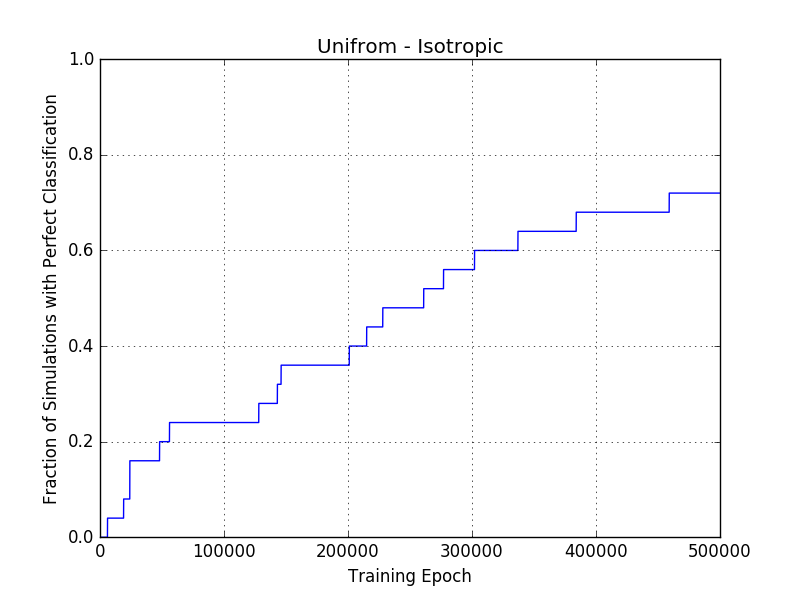
\includegraphics[width = 1.6in, trim={2.35cm 0 1.5cm 0.8cm},clip]{figures/completeFrac/completeFrac_u_i.png} \fixedlabel{block1d}{1d} \\ \\[-10pt]
		
		
		\rotatebox{90}{	\begin{tabular}[x]{@{}c@{} }   Uniform \\ Anisotropicity \end{tabular} }
		& 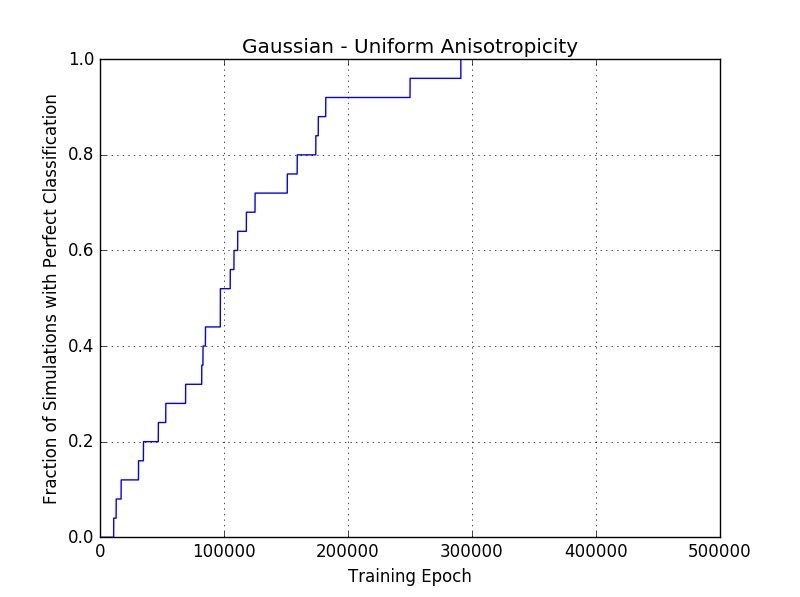
\includegraphics[width = 1.8in, trim={0.5cm 0 1.3cm 0.8cm},clip]{figures/completeFrac/completeFrac_g_ua.png} \fixedlabel{block2a}{2a} 
		& 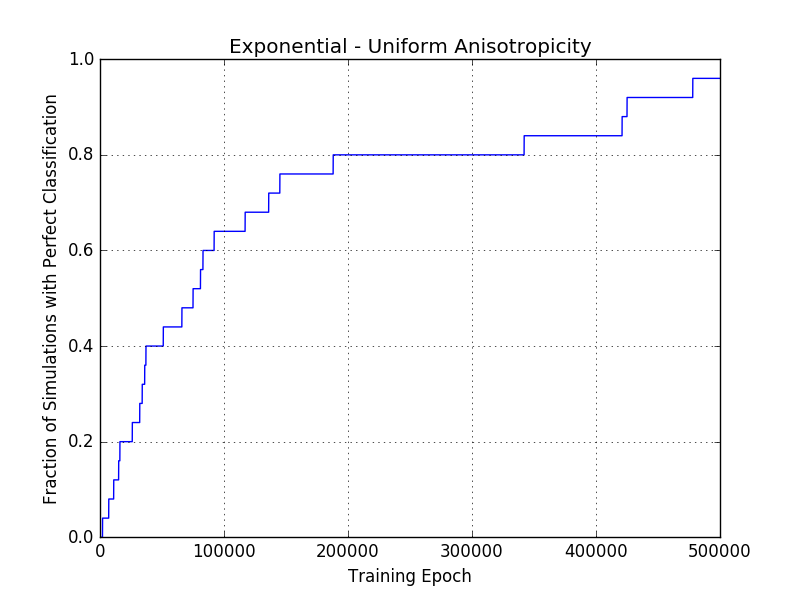
\includegraphics[width = 1.6in, trim={2.35cm 0 1.5cm 0.8cm},clip]{figures/completeFrac/completeFrac_e_ua.png} \fixedlabel{block1b}{2b} 
		& 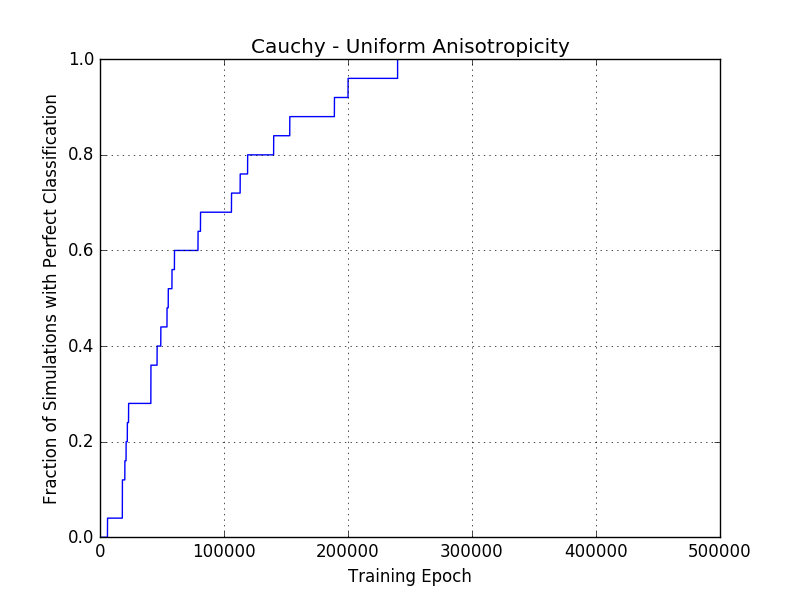
\includegraphics[width = 1.6in, trim={2.35cm 0 1.5cm 0.8cm},clip]{figures/completeFrac/completeFrac_c_ua.png} \fixedlabel{block1b}{2c} 
		& 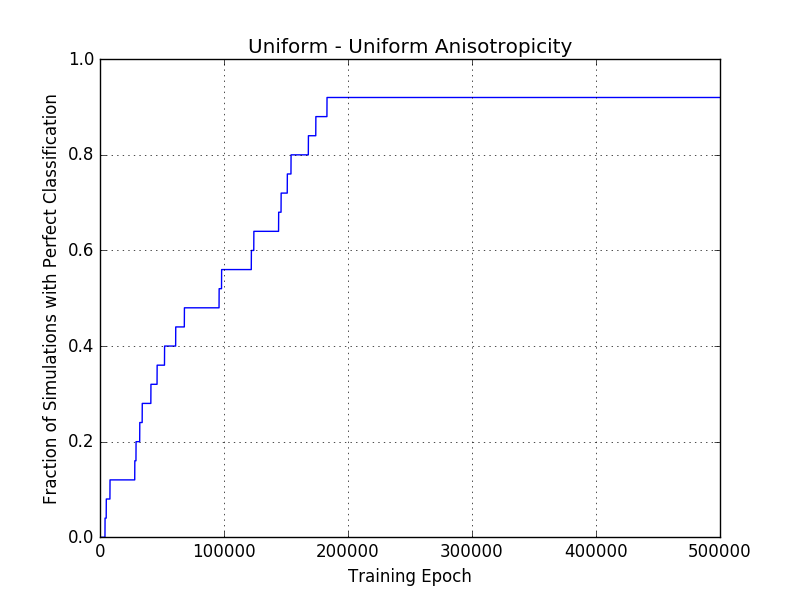
\includegraphics[width = 1.6in, trim={2.35cm 0 1.5cm 0.8cm},clip]{figures/completeFrac/completeFrac_u_ua.png} \fixedlabel{block2b}{2d} \\ \\[-10pt]
		
		\rotatebox{90}{	\begin{tabular}[x]{@{}c@{}} Variable \\ Anisotropicity \end{tabular}	}
		& 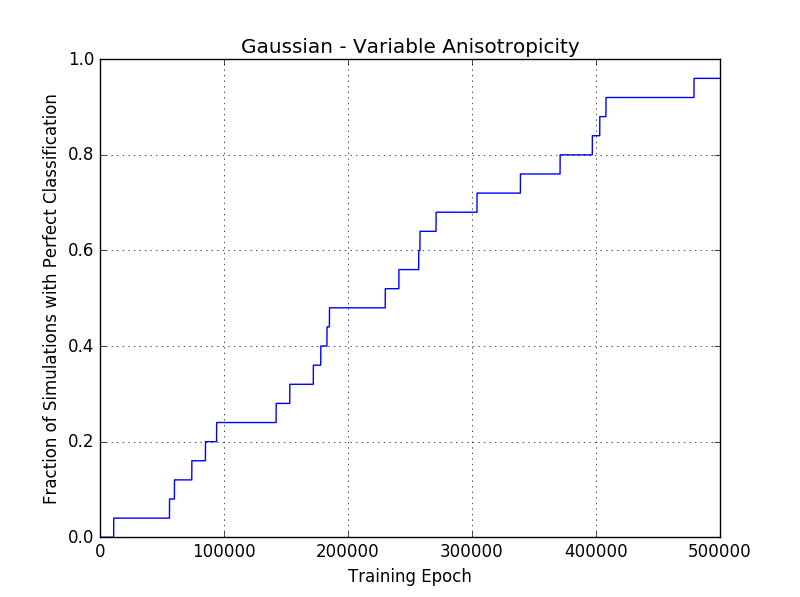
\includegraphics[width = 1.8in, trim={0.5cm 0 1.3cm 0.8cm},clip]{figures/completeFrac/completeFrac_g_va.png}\fixedlabel{block3a}{3a} 
		& 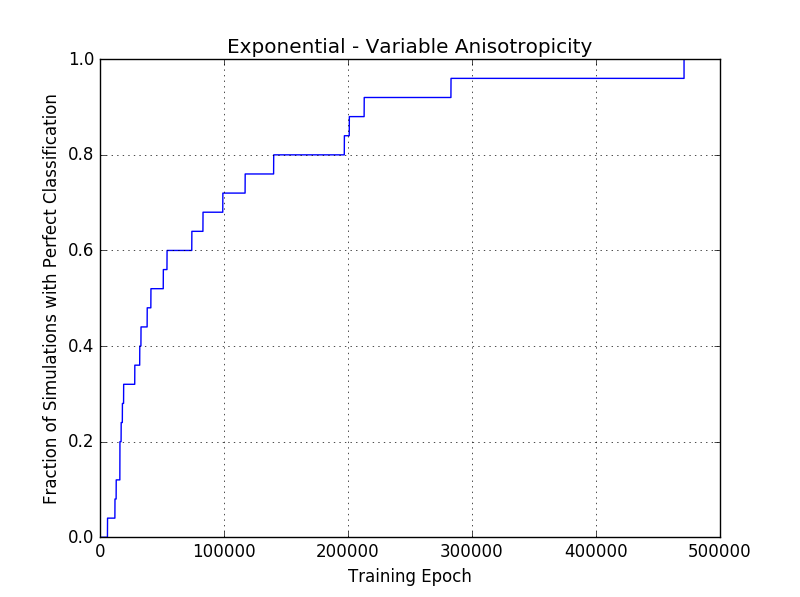
\includegraphics[width = 1.6in, trim={2.35cm 0 1.5cm 0.8cm},clip]{figures/completeFrac/completeFrac_e_va.png}\fixedlabel{block1b}{3b} 
		& 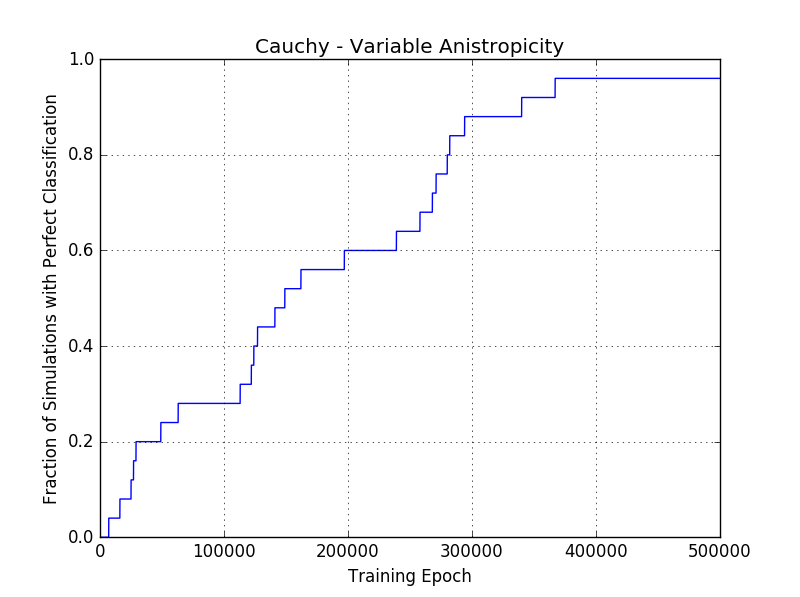
\includegraphics[width = 1.6in, trim={2.35cm 0 1.5cm 0.8cm},clip]{figures/completeFrac/completeFrac_c_va.png}\fixedlabel{block1b}{3c} 
		& 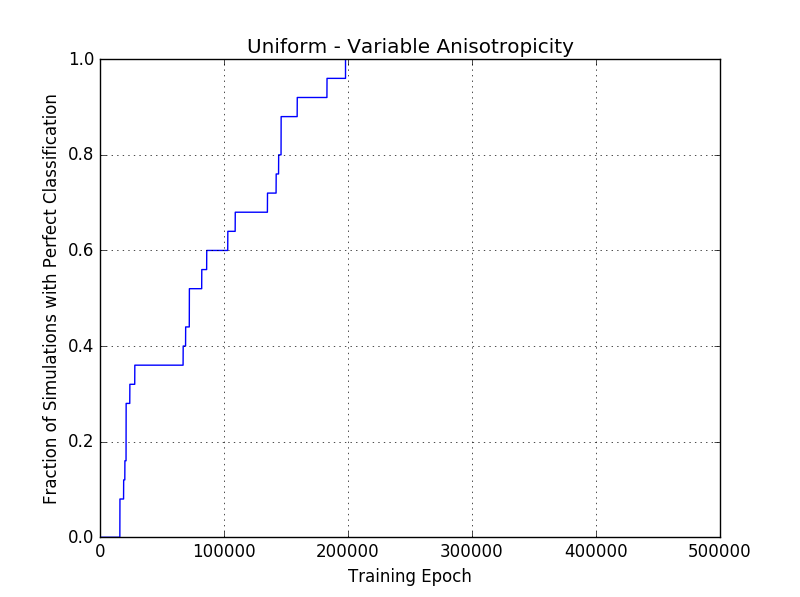
\includegraphics[width = 1.6in, trim={2.35cm 0 1.5cm 0.8cm},clip]{figures/completeFrac/completeFrac_u_va.png}\fixedlabel{block3b}{3d}
		
	\end{tabular}
	\caption{The simulation-time evolution of the fraction of 25 independent simulated annealing runs achieving perfect classification of Fishers iris data using a feed-forward neural network with 50 hidden units. Columns and rows are labeld as in Fig.~\ref{fig:class_perf}.}
\end{figure*}


\subsubsection{Perfect Classification Rate Analysis}

It is not possible to analyze the classification performance of individual SA trials in Fig.~\ref{fig:class_perf} because the classification performance is averaged. In order to analyze the performance of the individual trials more thoroughly Fig.~\ref{fig:perfect_class_time} shows the fraction of the 25 independent SA trails that have completed at each training epoch. The relative performance of the neighborhood functions are similar when compared using this metric, but we can gain additional insight from the new data. The fractional-completion data shows us that for almost all of the neighborhood functions the relationship between the simulation time and the fraction of trials achieving perfect classification is not linear. Instead, the relationship resembles a Gamma distribution cumulative distribution function. As such, we take the expectation value and standard deviation of the time required to reach a cost surface global minimum and use these values to complete the shape and scale parameters of the Gamma distribution. With the shape and scale parameters, it is possible to reconstruct the probability density function which approximates the PDF of the time to perfect classification.
 

These PDFs are useful because they can inform an important annealing technique: reannealing. As an annealing network traverses a cost surface it is possible for the system to become temporarily trapped in a basin which is far, in weight space distance, from the global minimum. As such, it is occasionally useful to increase, or rescale, the stochastic control parameters. It is suggested in \cite{ingber1989veryfastsimulatedreannealing} that the temperature be rescaled at approximately every hundred successful jumps. Though no reannealing schedule is presented in this paper, Figs.~\ref{fig:gaussian_gamma}, \ref{fig:exp_gamma}, \ref{fig:uniform_gamma}, and \ref{fig:cauchy_gamma} provide information regarding the optimal rescaling frequency for this classification problem. We suggest that the temperature rescaling interval which minimizes the average time required to reach a global minimum is the time at which the first inflection point of the perfect classification time PDF occurs. This choice of rescaling interval would ensure that the system constantly remains in the phase of the annealing process during which it has the greatest probability per unit time to reach a global minimum of the cost surface. This point corresponds to the expected value of the time to find the global minimum.

\begin{figure} 
	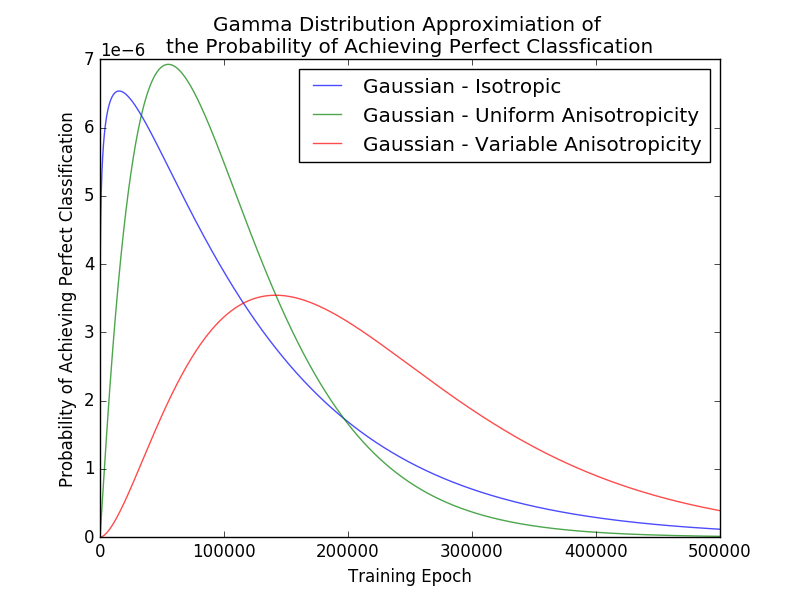
\includegraphics[width = 3.3in, trim={0.5cm 0 1.2cm 0.0cm},clip]{figures/gammaDists/gamma_g.png}
	\caption{This figure shows the gamma distribution approximations of the probability of achieving perfect classification through simulation time. This figure depicts the approximations for all Gaussian visiting distributions, and thus corresponds to the first column of Fig.~\ref{fig:perfect_class_time}}
	\label{fig:gaussian_gamma}
\end{figure}

\begin{figure} 
	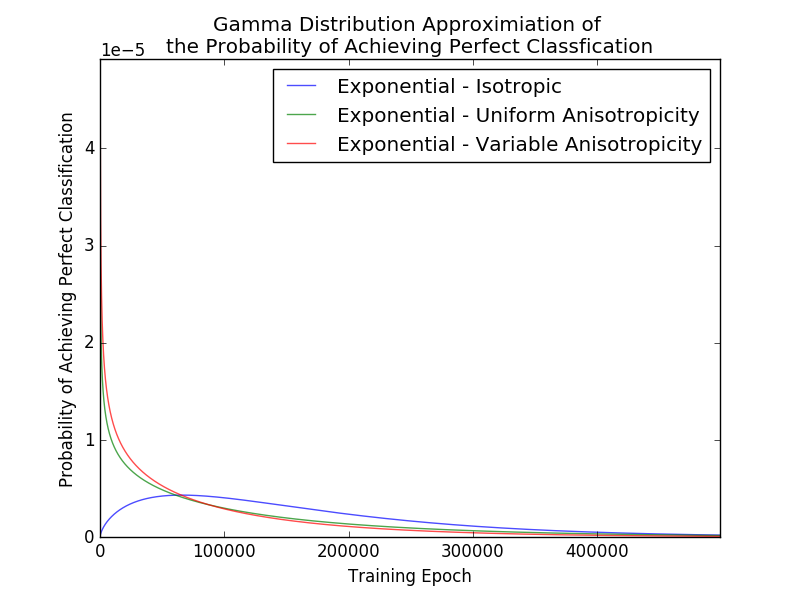
\includegraphics[width = 3.3in, trim={0.5cm 0 1.2cm 0.0cm},clip]{figures/gammaDists/gamma_e.png}
	\caption{This figure shows the gamma distribution approximations of the probability of achieving perfect classification through simulation time. This figure depicts the approximations for all  exponential visiting distributions, and thus corresponds to the second column of Fig.~\ref{fig:perfect_class_time}}
	\label{fig:exp_gamma}
\end{figure}

\begin{figure} 
	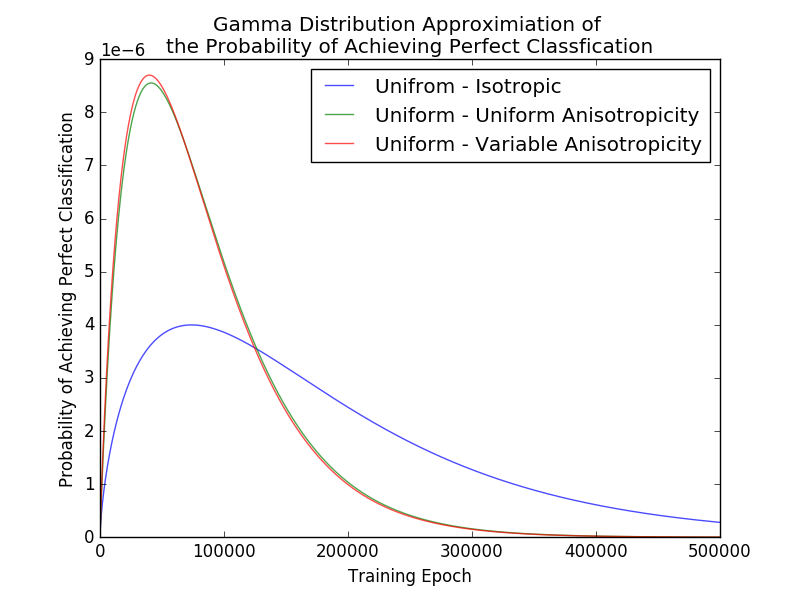
\includegraphics[width = 3.3in, trim={0.5cm 0 1.2cm 0.0cm},clip]{figures/gammaDists/gamma_u.png}
	\caption{This figure shows the gamma distribution approximations of the probability of achieving perfect classification through simulation time. This figure depicts the approximations for all uniform visiting distributions, and thus corresponds to the third column of Fig.~\ref{fig:perfect_class_time}}
	\label{fig:uniform_gamma}
\end{figure}

\begin{figure} 
	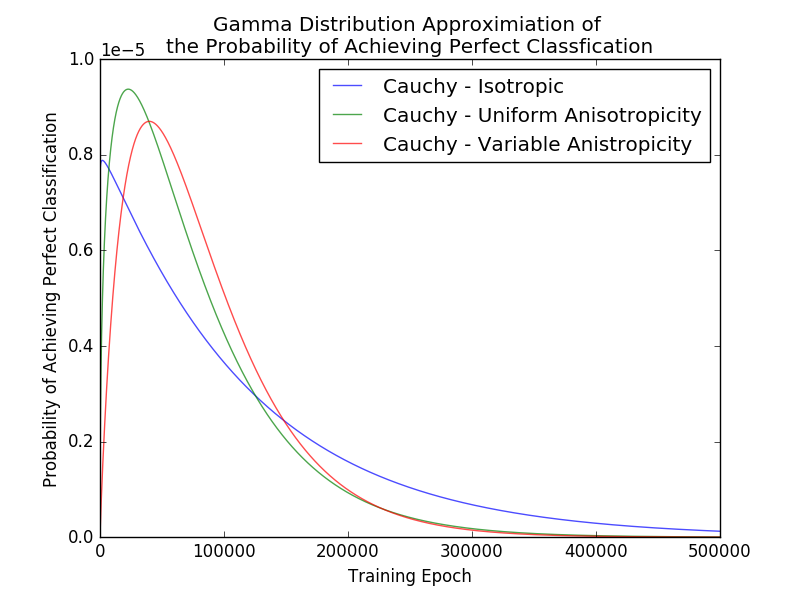
\includegraphics[width = 3.3in, trim={0.5cm 0 1.2cm 0.0cm},clip]{figures/gammaDists/gamma_c.png}
	\caption{This figure shows the gamma distribution approximations of the probability of achieving perfect classification through simulation time. This figure depicts the approximations for all Cauchy visiting distributions, and thus corresponds to the fourth column of Fig.~\ref{fig:perfect_class_time}}
	\label{fig:cauchy_gamma}
\end{figure}


\section{Conclusion}

We have proposed anisotropicity as a new simulated annealing neighborhood function parameter, presented a framework for applying simulated annealing to feed forward neural network weight selection, and numerically analyzed the performance of annealing systems constructed according to this framework. We have demonstrated that the anisotropicity of a neighborhood function can have a significant impact on the classification performance of a feed forward neural network.  

\label{scn:conclusion}

\bibliographystyle{IEEEtran}
\bibliography{synapticAnnealingBib}



\begin{IEEEbiography} {Justin R. Fletcher} %[{\includegraphics[width=1in,height=1.25in,clip,keepaspectratio]{figures/justin1.eps}}]
received the B.S degree in Computer Engineering from Embry-Riddle Aeronautical University in 2012 and is currently pursuing the M.S. degree in Computer Science from the Air Force Institute of Technology (AFIT). His research interests include neurocomputation, biologically-inspired computation, and computational physics.
\end{IEEEbiography}


\begin{IEEEbiography}{Michael J. Mendenhall} %[{\includegraphics[width=1in,height=1.25in,clip,keepaspectratio]{figures/mike1.eps}}]
	received the B.S. degree in Computer Engineering from Oregon State University, Corvallis, OR in 1996, the M.S. degree in Computer Engineering 
	from the Air Force Institute of Technology (AFIT), Wright-Patterson AFB, OH, in 2001, and the Ph.D. degree in Electrical Engineering from Rice 
	University, Houston, TX, in 2006. Currently, he is an Assistant Professor of Electrical Engineering at AFIT. He received the Dr. Leslie M. Norton 
	teaching award by the AFIT student association and an honorable mention for the John L. McLucas basic research award at the Air Force level, 
	both in 2010.  His research interests are in hyperspectral signal/image processing, hyperspectral signature modeling, and computational intelligence.  
\end{IEEEbiography}


\end{document}
